% template.tex, dated April 5 2013
% This is a template file for Annual Reviews 1 column Journals
%
% Compilation using ar-1col.cls' - version 1.0, Aptara Inc.
% (c) 2013 AR
%
% Steps to compile: latex latex latex
%
% For tracking purposes => this is v1.0 - Apr. 2013

\documentclass[letterpaper]{ar-1col}\usepackage[]{graphicx}\usepackage[]{color}
% maxwidth is the original width if it is less than linewidth
% otherwise use linewidth (to make sure the graphics do not exceed the margin)
\makeatletter
\def\maxwidth{ %
  \ifdim\Gin@nat@width>\linewidth
    \linewidth
  \else
    \Gin@nat@width
  \fi
}
\makeatother

\definecolor{fgcolor}{rgb}{0.345, 0.345, 0.345}
\newcommand{\hlnum}[1]{\textcolor[rgb]{0.686,0.059,0.569}{#1}}%
\newcommand{\hlstr}[1]{\textcolor[rgb]{0.192,0.494,0.8}{#1}}%
\newcommand{\hlcom}[1]{\textcolor[rgb]{0.678,0.584,0.686}{\textit{#1}}}%
\newcommand{\hlopt}[1]{\textcolor[rgb]{0,0,0}{#1}}%
\newcommand{\hlstd}[1]{\textcolor[rgb]{0.345,0.345,0.345}{#1}}%
\newcommand{\hlkwa}[1]{\textcolor[rgb]{0.161,0.373,0.58}{\textbf{#1}}}%
\newcommand{\hlkwb}[1]{\textcolor[rgb]{0.69,0.353,0.396}{#1}}%
\newcommand{\hlkwc}[1]{\textcolor[rgb]{0.333,0.667,0.333}{#1}}%
\newcommand{\hlkwd}[1]{\textcolor[rgb]{0.737,0.353,0.396}{\textbf{#1}}}%
\let\hlipl\hlkwb

\usepackage{framed}
\makeatletter
\newenvironment{kframe}{%
 \def\at@end@of@kframe{}%
 \ifinner\ifhmode%
  \def\at@end@of@kframe{\end{minipage}}%
  \begin{minipage}{\columnwidth}%
 \fi\fi%
 \def\FrameCommand##1{\hskip\@totalleftmargin \hskip-\fboxsep
 \colorbox{shadecolor}{##1}\hskip-\fboxsep
     % There is no \\@totalrightmargin, so:
     \hskip-\linewidth \hskip-\@totalleftmargin \hskip\columnwidth}%
 \MakeFramed {\advance\hsize-\width
   \@totalleftmargin\z@ \linewidth\hsize
   \@setminipage}}%
 {\par\unskip\endMakeFramed%
 \at@end@of@kframe}
\makeatother

\definecolor{shadecolor}{rgb}{.97, .97, .97}
\definecolor{messagecolor}{rgb}{0, 0, 0}
\definecolor{warningcolor}{rgb}{1, 0, 1}
\definecolor{errorcolor}{rgb}{1, 0, 0}
\newenvironment{knitrout}{}{} % an empty environment to be redefined in TeX

\usepackage{alltt}


\usepackage[comma]{natbib}
\bibliographystyle{ar-style1}

\setcounter{secnumdepth}{4}
% \usepackage{fullpage}
% \usepackage{lipsum}

\usepackage{graphicx}
\usepackage[hypcap=false]{caption}
\usepackage{hyperref}

% \usepackage{xcolor}
\definecolor{blue}{cmyk}{1,1,0,0}
\definecolor{pink}{cmyk}{0,1,0,0}
\definecolor{darkgreen}{cmyk}{0, .39, .97, 0}
\newcommand{\todo}[1]{\textcolor{pink}{#1}}
\newcommand{\svp}[1]{\textcolor{blue}{#1}}
\newcommand{\hh}[1]{\textcolor{darkgreen}{#1}}

\setcounter{secnumdepth}{4}

% Metadata Information
\jname{Xxxx. Xxx. Xxx. Xxx.}
\jvol{AA}
\jyear{YYYY}
\doi{10.1146/((please add article doi))}

% Document starts
\IfFileExists{upquote.sty}{\usepackage{upquote}}{}
\begin{document}
%\SweaveOpts{concordance=TRUE}

% Page header
\markboth{VanderPlas et al.}{Testing Statistical Charts}

% Title
\title{Testing Statistical Charts: What makes a good graph?}

%Authors, affiliations address.
% No idea how this should be ordered, so just doing it alphabetically for now :)
\author{Susan Vanderplas$^1$, Dianne Cook$^2$, and  Heike Hofmann$^3$
\affil{$^1$Statistics Department, Iowa State University, Ames, Iowa, United States, 50011; email: srvander@iastate.edu}
\affil{$^2$Econometrics and Business Statistics, Monash University, Melbourne,  Clayton VIC 3800, Australia}
\affil{$^3$Statistics Department, Iowa State University, Ames, Iowa, United States, 50011}}


%Abstract
\begin{abstract}
% Abstract text, approximately 150 words.
% \lipsum[3]
\end{abstract}

%Keywords, etc.
\begin{keywords}
keywords, separated by comma, no full stop, lowercase
\end{keywords}
\maketitle

%Table of Contents
\tableofcontents

% Heading 1
\section{INTRODUCTION}
% Graphics research is conducted across a wide range of research areas, from statistics and computer science to psychology, marketing, and communications. We will first consider the disciplines where this research is currently found as well as its historical origins (1.5 pages).
Any survey of literature on statistical charts and graphs will be complicated by the fragmentation of the literature, which occurs because any discipline which uses charts to summarize information generally also has individuals who research and assess the utility of these graphics. A quick survey reveals publications in journals from computer science, psychology, marketing and business, economics, ergonomics and human factors, statistics, sociology, communication and rhetoric, engineering, instructional design, and education. A review of early surveys of graphical forms suggests that this problem has long plagued the study of graphics, as \citet{funkhouserHistoricalDevelopmentGraphical1937} discusses the broad displines affected by statistical graphics and  \citet{kruskalVisionsMapsGraphs1977} addresses the difficulty of a comprehensive review of the relevant literature.

% \begin{quote}
% Whatever relates to extent and quantity may be represented by geometrical figures. Statistical projections which speak to the senses without fatiguing the mind, possess the advantage of fixing the attention on a great number of important facts." - Alexander von Humboldt, 1811, in \citet{funkhouserHistoricalDevelopmentGraphical1937}
% \end{quote}

Historically, the development of graphs and charts has been linked to the development of coordinate systems~\citep{fienbergGraphicalMethodsStatistics1979,benigerQuantitativeGraphicsStatistics1978,funkhouserHistoricalDevelopmentGraphical1937} and abstract representations of data. Preceding the development of formal mathematical coordinates, however, humanity has been representing information in abstract visual form since the origins of civilisation, e.g. spatial information using maps~~\citep{smithImagoMundiLogo1996} are displayed with varying degrees of abstraction. \autoref{fig:imagomundi} shows the oldest known world map, which dates from 6th century BCE Babylon. %\svp{there has to be a better transition here, but I've spent too much time on it to bother right now}

\begin{minipage}{.35\textwidth}

\includegraphics[width=\textwidth]{figure/ImagoMundi.jpg}
\end{minipage}\hfill
\begin{minipage}{.6\textwidth}
\captionof{figure}{Imago Mundi Babylonian map, which is the oldest known world map (6th centure BCE). The representation of the world is relatively abstract. The world is shown as a disc, with Babylon represented by a rectangle lat the right end of the Euphrates river, which flows south to the border of the disc. Several other population centers are marked with small circles.~\citep{imagomundi}\\{\small Image courtesy of the British Museum, released under a CC By-NC-SA 4.0 license.}}\label{fig:imagomundi}
\end{minipage}
Exploring visual abstractions of data, has been an active pursuit of the ``polymaths" who, grappling with increasing collections of economic, demographics, and measurements on the natural world, developed the foundations of current scientific pursuits. During the 18$^{th}$ and 19$^{th}$ centuries, governments became involved, assembling data and graphical representations into the statistical atlases, and government issued reports, as created by \citet{Crome}, \citet{playfair1801statistical}, \citet{atlas}, and many other contemporary workman. In the 20th century, corporations began using charts and graphs to understand their inner workings - studies of the use of charts and graphs at AT\&T~\citep{chandarGraphStandardizationManagement2012} and DuPont~\citep{yatesGraphsManagerialTool1985a} show efforts to standardize and formalize the use of graphics in decision-making at both companies.

As new charts were invented to represent data differently and highlight features of data~\citep{bernsteinGraphicPresentationTrend1937,yatesGraphsManagerialTool1985a,mcdonaldFlorenceNightingaleStatistics2014}, discussions about the use of statistical graphics began to appear in the literature~\citep{peuchet1805statistique,brinton1917graphic,karsten1923charts}, including the relative strengths and weaknesses of various types of charts. In most cases, the drive to produce a classification system for charts and graphs or a system of recommendations for presenting charts and graphs were  based on heuristics and largely unsupported by experimentation~\citep{kruskalVisionsMapsGraphs1977,macdonald-rossHowNumbersAre1977}. Many of these ad-hoc classification systems could not accommodate the large numbers of new plot types being developed.

\begin{marginnote}
% \begin{quote}
All the graphic methods enumerated already exist and it is unlikely that
a completely new one will be invented. Since they have been used separately
up until the present time it would be convenient to classify them by analogy,
according to the categories above...
- \citet{EmploiCartographieMethode1858}, in \citet{funkhouserHistoricalDevelopmentGraphical1937}
% \end{quote}
\end{marginnote}

%\todo{Need better transitions here between playfair and experimental graphics. Should probably discuss Tukey, the rise of computer generated graphics...}

Calls for experimental validation of the perception and utility of statistical charts were heeded, though at first the experiments were fraught with methodological issues~\citep{croxtonBarChartsCircle1927}. Much of the early experimentation regarding the accuracy of graphical forms was based in psychophysics research~\citep{teghtsoonian_judgment_1965} on the perception of size and shape. Eventually experiments became more naturalistic: cognitive psychologists and statisticians began testing different types of graphics, identifying types of perceptual errors associated with different plots~\citep{spenceVisualPsychophysicsSimple1990,cleveland_graphical_1985}. In most cases, this testing was limited to simply reading information from the charts, using accuracy or response time measurement. More recently, other methods for examining statistical charts have been developed, including the lineup protocol~\citep{wickhamGraphicalInferenceInfovis2010}. Even with these developments, the aim of most experimental research in statistical graphics focuses on the initial perception and graph comprehension. Very little work has been done to understand the effect of charts and graphs on higher cognitive processes such as learning or analysis~\citep{greenPersonalEquationComplex2011}.

\subsection{Design of Statistical Graphics}
% We will also discuss the different approaches to graphical design, ranging from utilitarian charts used for quick data presentation to artistic renderings which encourage aesthetics over utility (2 pages).


Charts and graphs are used for many purposes~\citep{tukeyGraphicSemigraphicDisplays1972,fienbergGraphicalMethodsStatistics1979}: to summarize data, for analysis, exploration and discovery, diagnosis of statistical relationships, to make a rhetorical argument, or even as a substitute for tables. The initial heyday of graphic design was enabled by colour lithography used charts and graphs to tell stories about nations and events~\citep{kostelnickReEmergenceEmotionalAppeals2016}, but in the first half of the 20th century, graphics were regularly used for mundane purposes as well, such as supporting business decisions~\citep{chandarGraphStandardizationManagement2012,yatesGraphsManagerialTool1985a} and communicating weather forecasts. As technology has developed, allowing charts to be created quickly for exploratory purposes, the gaps between graphics for presentation, entertainment, and analysis have widened. The different purposes motivating the creation of the chart influence the form and complexity of the chart, and the intended audience and the reach of the chart are also important considerations.

It is useful to consider a continuum from utilitarianism to artistry, where purely utilitarian charts are, as advocated by \citet{tufte}, devoid of ``chartjunk" or any decoration, and purely artistic charts trade accurate representation of the data for visually compelling renderings. The distinction between infographics and statistical graphics is primarily one of intent: the infographic, often composed of many small simple plots interspersed with pictures and text, is designed to attract attention and tell a story. In contrast, the statistical chart is designed to effectively and accurately show the data, potentially with accompanying statistical model information -- any visual enhancements should contribute to that aim~\citep{gelmanInfovisStatisticalGraphics2013,wickham2013graphical}.

Figures \ref{fig:hrdiagram}, \ref{fig:noaa-michael} and \ref{fig:bdaychart} show plots designed for different statistical purposes. The Hertzsprung-Russell diagram allowed astrophysicists to make a convincing argument about the lifecycle of a star, based on its temperature, colour, and size. The hurricane forecast map is designed to communicate urgent information and facilitate decision-making by the US National Hurricane Center. It shows forecasts of the hurricane's path, the wind field, forecasted strength, and coastal warnings. \autoref{fig:noaa-michael} shows the prediction map for Hurricane Michael, which hit the Florida panhandle in October 2018. It is primarily utilitarian, with additional decorations such as ocean colour and state boundaries provided for geographic context. The birthday chart reproduced in \autoref{fig:bdaychart} shows the average number of births in the United States on each day of the year, organized by month. \autoref{fig:bdaychart} is a static reproduction of an  interactive plot used as part of a web page (\url{http://thedailyviz.com/2016/09/17/how-common-is-your-birthday-dailyviz/}) telling a story about birth dates. It is simple in form, almost infographic style. By engaging with the interactive chart, a reader could easily deduce that there are relatively few babies born on major holidays, such as Memorial Day, Independence Day, and Christmas; there are also considerably more babies born in the summer months than in the winter.



% \todo{use \citet{byrneAcquiredCodesMeaning2016} to assess data visualization vs. infographics}

% Sample plots for some of these purposes might be good - HR diagram (discovery/analysis), Minard/Napoleon (rhetorical argument), pie chart or mosaic plot from the statistical atlas or a pictoral chart as in Vernon (1946) (table substitute), data summary (some sort of process control chart? - dupont?)


\begin{minipage}{.45\textwidth}
\centering
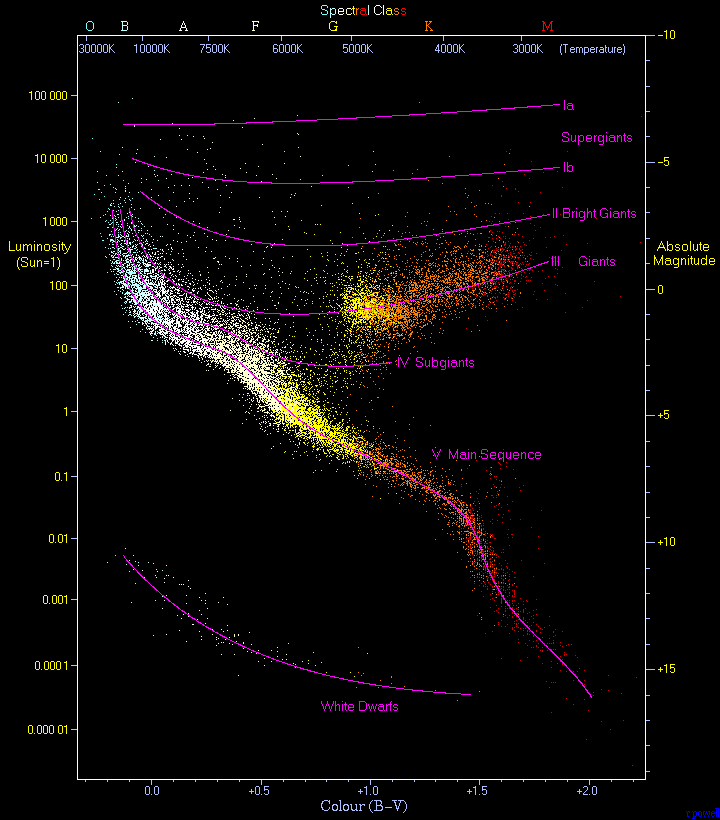
\includegraphics[width=.98\textwidth]{figure/HRDiagram.png}
\captionof{figure}{The Hertzsprung-Russell diagram (circa 1910) allowed astrophysicists to make the connection between a star's temperature, visual colour, and size, enabling a better understanding of the life cycle of a star.}\label{fig:hrdiagram}
\end{minipage}\hfill
\begin{minipage}{.45\textwidth}
\centering
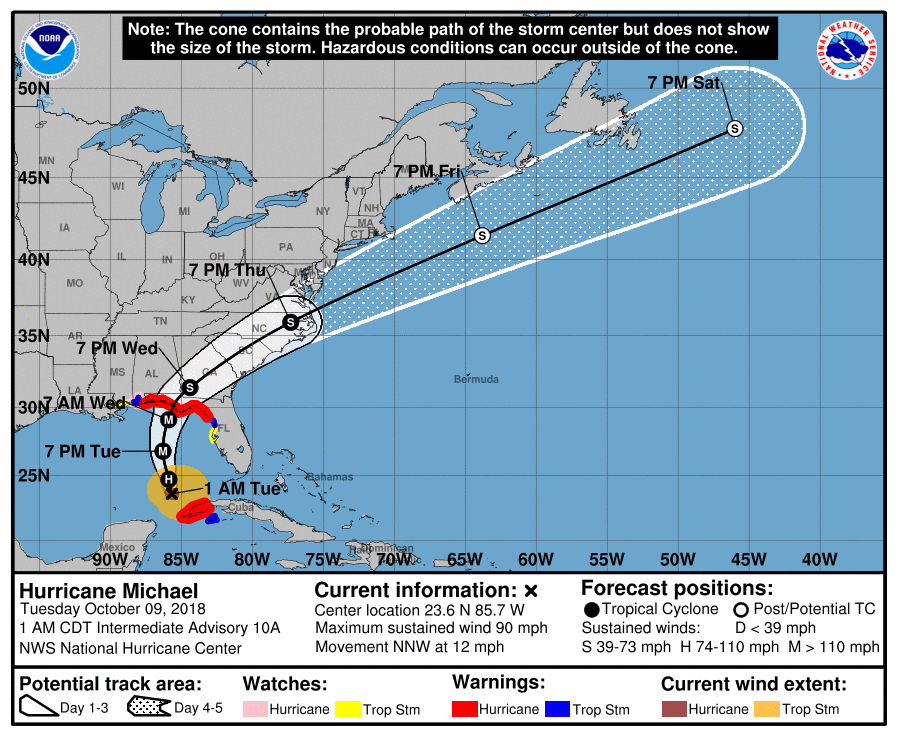
\includegraphics[width=.98\textwidth]{figure/noaa_michael.png}
\captionof{figure}{Hurricane forecast map issued on October 9, 2018, shortly before Hurricane Michael made landfall in the Florida panhandle. The predicted hurricane path, wind field size, and coastal weather status allow consumers to make educated decisions about evacuation orders.}\label{fig:noaa-michael}
\end{minipage}

\begin{knitrout}
\definecolor{shadecolor}{rgb}{0.969, 0.969, 0.969}\color{fgcolor}\begin{figure}
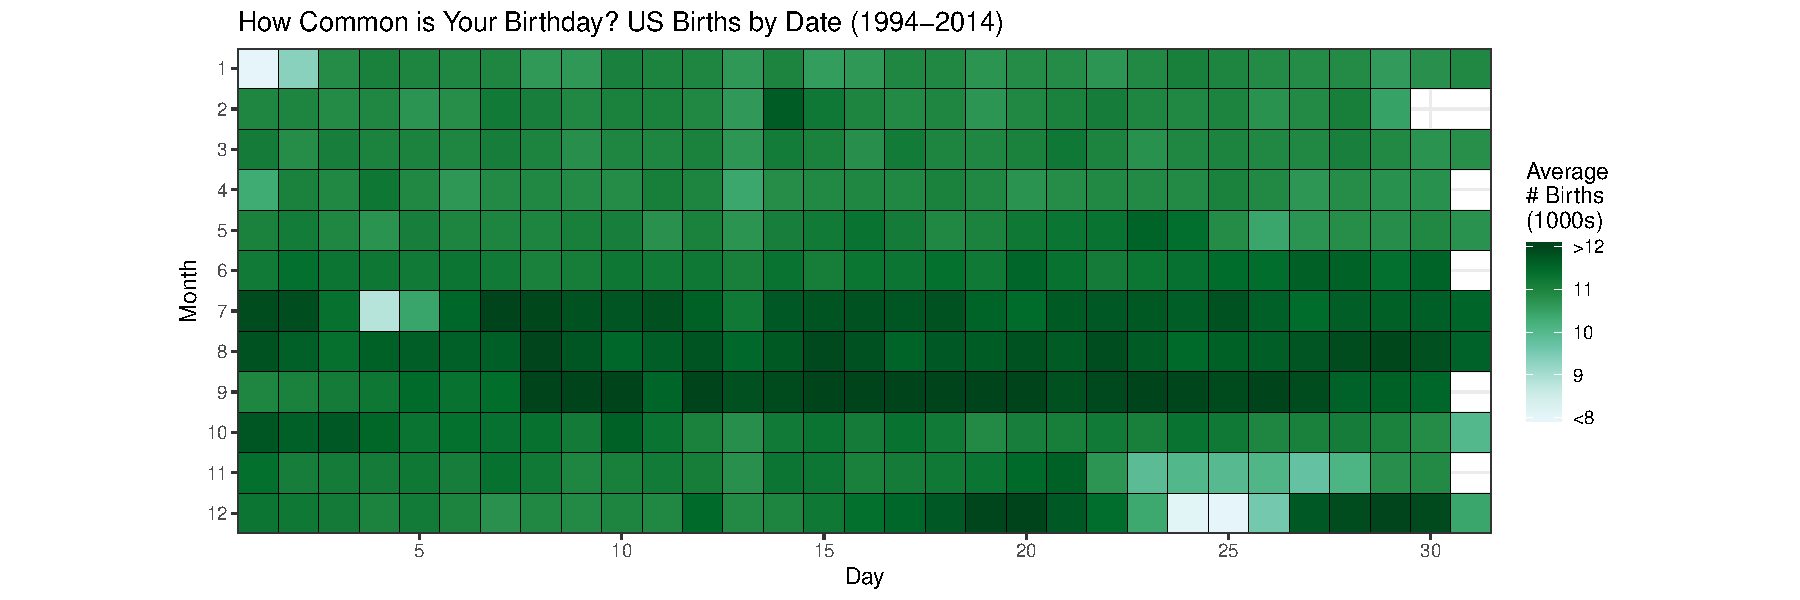
\includegraphics[width=1.3\linewidth]{figure/bdaychart-1} \caption{A static reproduction of the birthday chart, which shows the average number of births on a yearly basis in the United States, by month and day of the month. The interactive version, available at \url{http://thedailyviz.com/2016/09/17/how-common-is-your-birthday-dailyviz/}, is designed to be a storyteller to encourage the viewer to interact, check the estimated conception dates and read the frequency. Data source: CDC National Center for Health Statistics (1994-2003) and Social Security Administration (2000-2014), as reproduced at \url{https://github.com/fivethirtyeight/data/tree/master/births}.}\label{fig:bdaychart}
\end{figure}


\end{knitrout}

\subsection{Statistical Mapping Using a Grammar of Graphics}
%We will also highlight the grammar of graphics as an important development which facilitates scientific analysis of statistical graphics by separating the physical representation from the underlying data (3 pages).

In parallel with efforts to understand the perception of charts, there have been many attempts to develop systems for classifying graphics, including \citet{bertin1983semiology}, \citet{desnoyersTaxonomyVisualsScience2011}, and \citet{wilkinson1999grammar}. Systems which attempt to categorize charts based on their geometric representations generally make no effort to include all types of graphics, and have difficulty accommodating charts which may fall into two or more categories. The classification of graphics based on the underlying components and their relationships, as in the grammar of graphics developed by \citeauthor{wilkinson1999grammar} are more robust; they also provide an elegant framework for comparing different types of graphical representations separate from the underlying data structure. An analogy to conceptualise the difference is that the former is like treating plots like creatures in a zoo, with a unique name for each, while the latter is analgous to having a phylogeny based on genetic data showing how plots are related.

\autoref{fig:grammar-graphics-flowchart} shows the framework of the grammar of graphics, where the data is filtered, variables are mapped, transformations are specified, and then finally, transformed data are mapped to plot aesthetics and coordinate system specifications to produce an abstract visual representation of the data. Full or partial implementations of the grammar of graphics are available for most common scientific computing languages: e.g.\ \texttt{ggplot2} in R~\citep{wickhamLayeredGrammarGraphics2010}, \texttt{plotnine}, a python implementation of \texttt{ggplot2}~\citep{plotnine2017}, and \texttt{Gramm} in Matlab~\citep{morelGrammGrammarGraphics2018}.

\begin{figure}
\centering
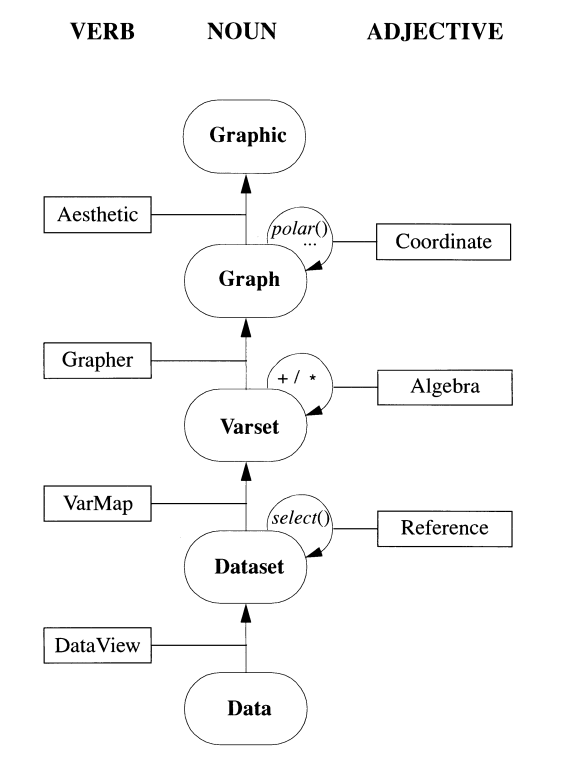
\includegraphics[width=.5\textwidth]{figure/grammar-graphics-flowchart}
\caption{From data to graphic, from~\citep[Fig 2.1]{wilkinson1999grammar}. The schematic representation of the steps required to create a graphic from a dataset, which can be used to specify the variable mapping, data transformations, coordinate system, and aesthetic features independently.}\label{fig:grammar-graphics-flowchart}
\end{figure}

The grammar of graphics also enables data plots to be considered to be statistics~\citep{majumderValidationVisualStatistical2013}. A statistic is a functional mapping of a variable or set of variables. With ``tidy data", that is, data where each variable is in its own column, each observation is in its own row, and each value is in its own cell~\citep{Wickham:2017:RDS:3086927}, the grammar of graphics creates visual statistics. Variables, as columns in the data table, are mapped to graphical elements, such as the $x$ axis, or $y$ axis, or to colour, shape or even facet, using the grammar. The data plot can then be treated like other statistics: by imagining what the plot might look like in the absence of of any structure, we can use the plot of the actual observed data to test for the likelihood of any perceived structure being significant.

Using the grammar of graphics, it is easy for experimenters to compare different types of charts using the same data, as the underlying structure of the graph remains the same. \autoref{fig:grammar-graphics-plots} shows three plots created using the same data and different geometric objects, with the \texttt{ggplot2} code to create the plots. Comparing these graphics experimentally would be reasonably simple as the grammar of graphics helps to control the extraneous variables introduced by utilizing different plot types. In addition, this approach to transformations and scales allows experimenters to easily test judgments made utilizing different axis transformations and colour scales to compare perceptual accuracy~\citep{hofmannGraphicalTestsPower2012,vanderplasClustersBeatTrend2017}.



\begin{figure}
\begin{minipage}{.495\textwidth}
\begin{knitrout}
\definecolor{shadecolor}{rgb}{0.969, 0.969, 0.969}\color{fgcolor}\begin{kframe}
\begin{alltt}
\hlcom{# Density plot}
\hlkwd{ggplot}\hlstd{(}\hlkwc{data} \hlstd{= banknote,}
       \hlkwd{aes}\hlstd{(}\hlkwc{x} \hlstd{= Bottom,}
           \hlkwc{group} \hlstd{= Type,}
           \hlkwc{fill} \hlstd{= Type))} \hlopt{+}
  \hlkwd{geom_density}\hlstd{(}\hlkwc{position} \hlstd{=} \hlstr{"stack"}\hlstd{)}
\end{alltt}
\end{kframe}
\end{knitrout}
\end{minipage}\hfill
\begin{minipage}{.45\textwidth}
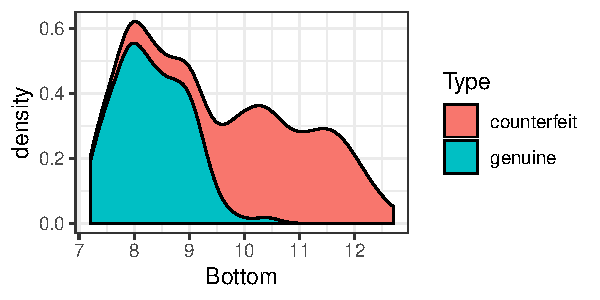
\includegraphics[width=.99\textwidth]{figure/gg-plots-figs-1}
\end{minipage}\\
\begin{minipage}{.495\textwidth}
\begin{knitrout}
\definecolor{shadecolor}{rgb}{0.969, 0.969, 0.969}\color{fgcolor}\begin{kframe}
\begin{alltt}
\hlcom{# Dotplot}
\hlkwd{ggplot}\hlstd{(}\hlkwc{data} \hlstd{= banknote,}
       \hlkwd{aes}\hlstd{(}\hlkwc{x} \hlstd{= Bottom,}
           \hlkwc{group} \hlstd{= Type,}
           \hlkwc{fill} \hlstd{= Type))} \hlopt{+}
  \hlkwd{geom_dotplot}\hlstd{(}\hlkwc{method} \hlstd{=} \hlstr{'histodot'}\hlstd{,}
               \hlkwc{stackgroups} \hlstd{=} \hlnum{TRUE}\hlstd{)}
\end{alltt}
\end{kframe}
\end{knitrout}
\end{minipage}\hfill
\begin{minipage}{.45\textwidth}
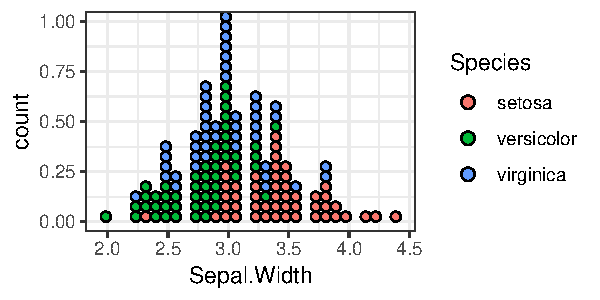
\includegraphics[width=.99\textwidth]{figure/gg-plots-figs-2}
\end{minipage}\\
\begin{minipage}{.495\textwidth}
\begin{knitrout}
\definecolor{shadecolor}{rgb}{0.969, 0.969, 0.969}\color{fgcolor}\begin{kframe}
\begin{alltt}
\hlcom{# Histogram}
\hlkwd{ggplot}\hlstd{(}\hlkwc{data} \hlstd{= banknote,}
       \hlkwd{aes}\hlstd{(}\hlkwc{x} \hlstd{= Bottom,}
           \hlkwc{group} \hlstd{= Type,}
           \hlkwc{fill} \hlstd{= Type))} \hlopt{+}
  \hlkwd{geom_histogram}\hlstd{(}\hlkwc{position} \hlstd{=} \hlstr{"stack"}\hlstd{)}
\end{alltt}
\end{kframe}
\end{knitrout}
\end{minipage}\hfill
\begin{minipage}{.45\textwidth}
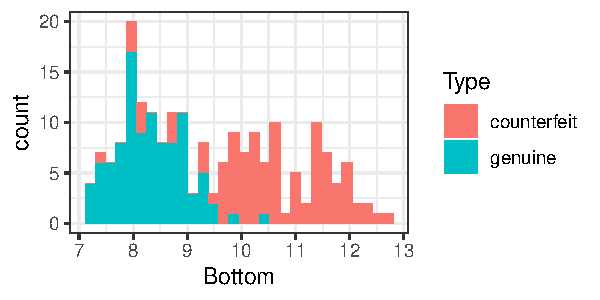
\includegraphics[width=.99\textwidth]{figure/gg-plots-figs-3}
\end{minipage}
\caption{Three different plots of the Swiss banknote data~\citep{banknote}, created using the grammar of graphics as implemented in \texttt{ggplot2}. The data consist of measurements of the dimensions of the banknotes, including the length of the bottom edge, which is shown in the plots. The main plot specification and syntax remain the same, with the form of the plot changing due to the specification of the geometric object used to represent the data.}\label{fig:grammar-graphics-plots}
\end{figure}
% \texttt{Vega-Lite}, a JSON graph specification schema~\citep{satyanarayanVegaLiteGrammarInteractive2017} which incorporates interactivity, \texttt{Altair}, a python implmementation built on Vega-Lite~\citep{vanderplasAltairInteractiveStatistical2018},

%\svp{Still need another page of content here...}

\section{TESTING METHODS} % 8 pages
% In this section, we will examine the methods which are used for testing statistical graphics experimentally. We will divide this discussion into two main sections: explicitly structured tests, where the experimenter must ask specific questions about the content of the charts and graphs under examination, and implicitly structured tests, where the participant must identify questions of interest from the provided stimuli.

% In the discussion of the importance of empirical testing of charts and graphs, \citet{kruskalVisionsMapsGraphs1977} list 3 main criteria for good a good experiment involving statistical graphics: \begin{enumerate}\item Testing should be in collaboration with good psychologists, \item it should be based on proper experimental designs, and \item it should lead to usable perceptual theory for the future.\end{enumerate} % not wild about the way this is phrased, but I like his criteria given the studies that were available at the time...
In this section, we will distinguish between explicitly structured graphical tests, which require the participants to answer specific questions about the graphical objects under experimentation, and implicitly structured tests, where the participant must infer the questions of interest from the provided stimuli.

% Heading 2
\subsection{Explicitly Structured Graphical Tests} % 3-4 pages
% We will briefly discuss experiments involving preattentive graph perception (1 page), but the remainder of the section will be devoted to attention-mediated testing methods, including numerical estimation (1 page), interactive adjustment (0.5 pages), think-aloud protocols (0.5 pages), and eye tracking (0.5 pages).

During the perceptual process, information from a visual scene is processed by the brain, with information extracted at many different levels of the cognitive process. Preattentive perceptual effects are those which do not require sustained cognitive attention; they are processed automatically within the first 500 milliseconds of viewing a chart or graph. Components processed preattentively include colour and shape, as well as some basic information about coarse relationships between individual components. After the preattentive stage, attention is necessary for subsequent processing; this directed attention scaffolds relationships between components and helps us interpret the chart or graph in context. Most of the insights we gain from charts and graphs are due to the cognitive processes that occur after attention is focused on specific aspects of the graph; as a result, most of the testing methods we will discuss are focused on the attentive portion of the perceptual process.

\subsubsection{Preattentive Graph Perception} % 1 page

Initial research into preattentive perception used a search task, where participants had to identify a particular object in a field of distractors, manipulating display size and varying one or more features such as colour or shape; participants' search times were measured to determine the amount of effort necessary to complete the search task. Preattentively perceived features showed a near constant reaction time over increasing display size, while features which are processed attentively show an increasing reaction time with increased display size~\citep{treismanFeatureIntegrationTheoryAttention1980}. A primary question in the discussion of preattentive graph perception is whether there are advantages in designing a graph to promote the preattentive perception of features, ideally, reducing cognitive load.




\noindent\begin{figure}
\begin{minipage}[c]{.575\textwidth}
\centering
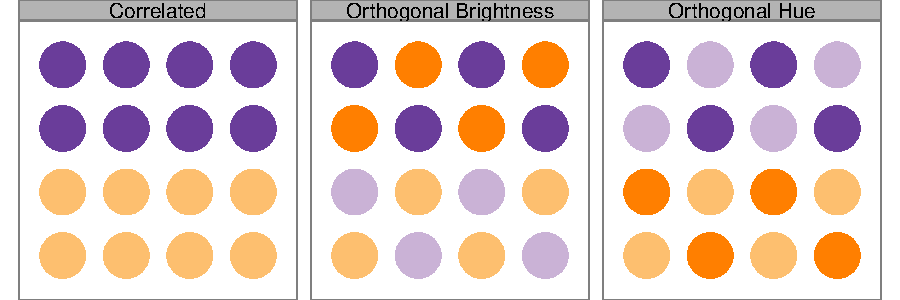
\includegraphics[width=\textwidth]{figure/hue-brightness-array-1}
\end{minipage}\hfill
\begin{minipage}[c]{.4\textwidth}
\caption{\citet{callaghanDimensionalInteractionHue1984} showed irrelevant variation increases response times, indicating that hue and brightness are integrated and preattentively perceived. The images shown here are examples of the types of stimuli used in the experiment. While hue and brightness can be manipulated separately, they are preattentively perceived as a single unit.}\label{fig:hue-brightness-array}
\end{minipage}
\end{figure}
We will distinguish between tests which use graphical forms and more primitive tests which use basic geometric elements during the testing process. The results from more primitive experimental designs still apply to the design of graphs and charts, but the experimental design does not involve any display of actual data (\autoref{fig:hue-brightness-array} is an example of an experimental stimuli that does not represent actual data). Preattentively processed features include shape, angle, size, and texture; however, typically, combinations of preattentive features which represent separate features in the data are processed attentively, with at least one major exception. \citet{callaghanDimensionalInteractionHue1984} demonstrated that hue and brightness are integrated, that is, that even though they can be separately manipulated, they are still perceived preattentively as a single unit, using arrays of tiles similar to those shown in \autoref{fig:hue-brightness-array}.

Extending this work, \citet{healeyHighspeedVisualEstimation1996} has used the same segmentation paradigm, applied to more complex charts utilizing actual data, with the goal of exploring region segmentation using preattentive cues. Healey's experiments use multivariate displays, leveraging the preattentive grouping of similar objects to separately represent features using colour, height, and texture~\citep{healeyLargeDatasetsGlance1999}. While these displays may not follow best graphical practice in other respects, % sorry, can't resist
they do show the utility of designing with the preattentive perceptual process in mind.

\subsubsection{Attention Mediated Testing Methods}
Creators of a chart or graph typically operate under the (hopefully safe) assumption that readers will spend more than 300 milliseconds considering its contents; as a result, attention mediated testing methods allow a more realistic mechanism for testing overall performance of different graphical forms. \citet{clevelandGraphicalPerceptionVisual1987} discuss the different approaches to research methodology in this area, and while they do not include all of the experimental approaches we discuss, the paper makes an important distinction between informal and formal graphical exploration. In the informal approach, changes are made to the graph and the iterative versions are compared to determine what information is easily accessible; in the formal approach, an experiment is designed and participants are tested in a controlled manner. This section describes several different experimental approaches which can be used to answer the general question of ``how effective is this graph at communicating useful information?"

\paragraph{Direct Observation: Numerical Estimation, Speed, and Error Rates} % 1 page
One of the simplest ways to test the utility of a graph is to verify that information can be accurately read from it. Charts are, after all, generally recognized as having more utility than tables for presenting information in an accessible and useful way; if that information cannot be read back out in a relatively accurate manner, the graph's utility is suspect. Early experiments, such as \citet{eellsRelativeMeritsCircles1926}, \citet{croxtonBarChartsCircle1927} and \citet{croxtonGraphicComparisonsBars1932} used accuracy alongside speed and other considerations for plot evaluation. Later studies~\citep{petersonHowAccuratelyAre1954,cleveland_graphical_1984,broersmaGraphicalPerceptionDistributional,dunnFramedRectangleCharts1988,tanHumanProcessingTwodimensional1994,amerBiasDueVisual2005} were conducted with similar methodology; in essence, the participants are provided with a chart and asked to estimate some quantity or answer a predefined question using the information provided in the chart. The accuracy of various types of charts, as measured by participants responses to the questions, is then used to determine which charts are superior. It is important to ensure that the specific charts and questions used are aligned; studies are commonly critiqued on the basis that the charts or the questions were not appropriate for the task  --- indeed, the first studies of pie vs. bar charts were heavily criticized on these grounds~\citep{vonhuhnFurtherStudiesGraphic1927}.

\begin{minipage}{.4\textwidth}
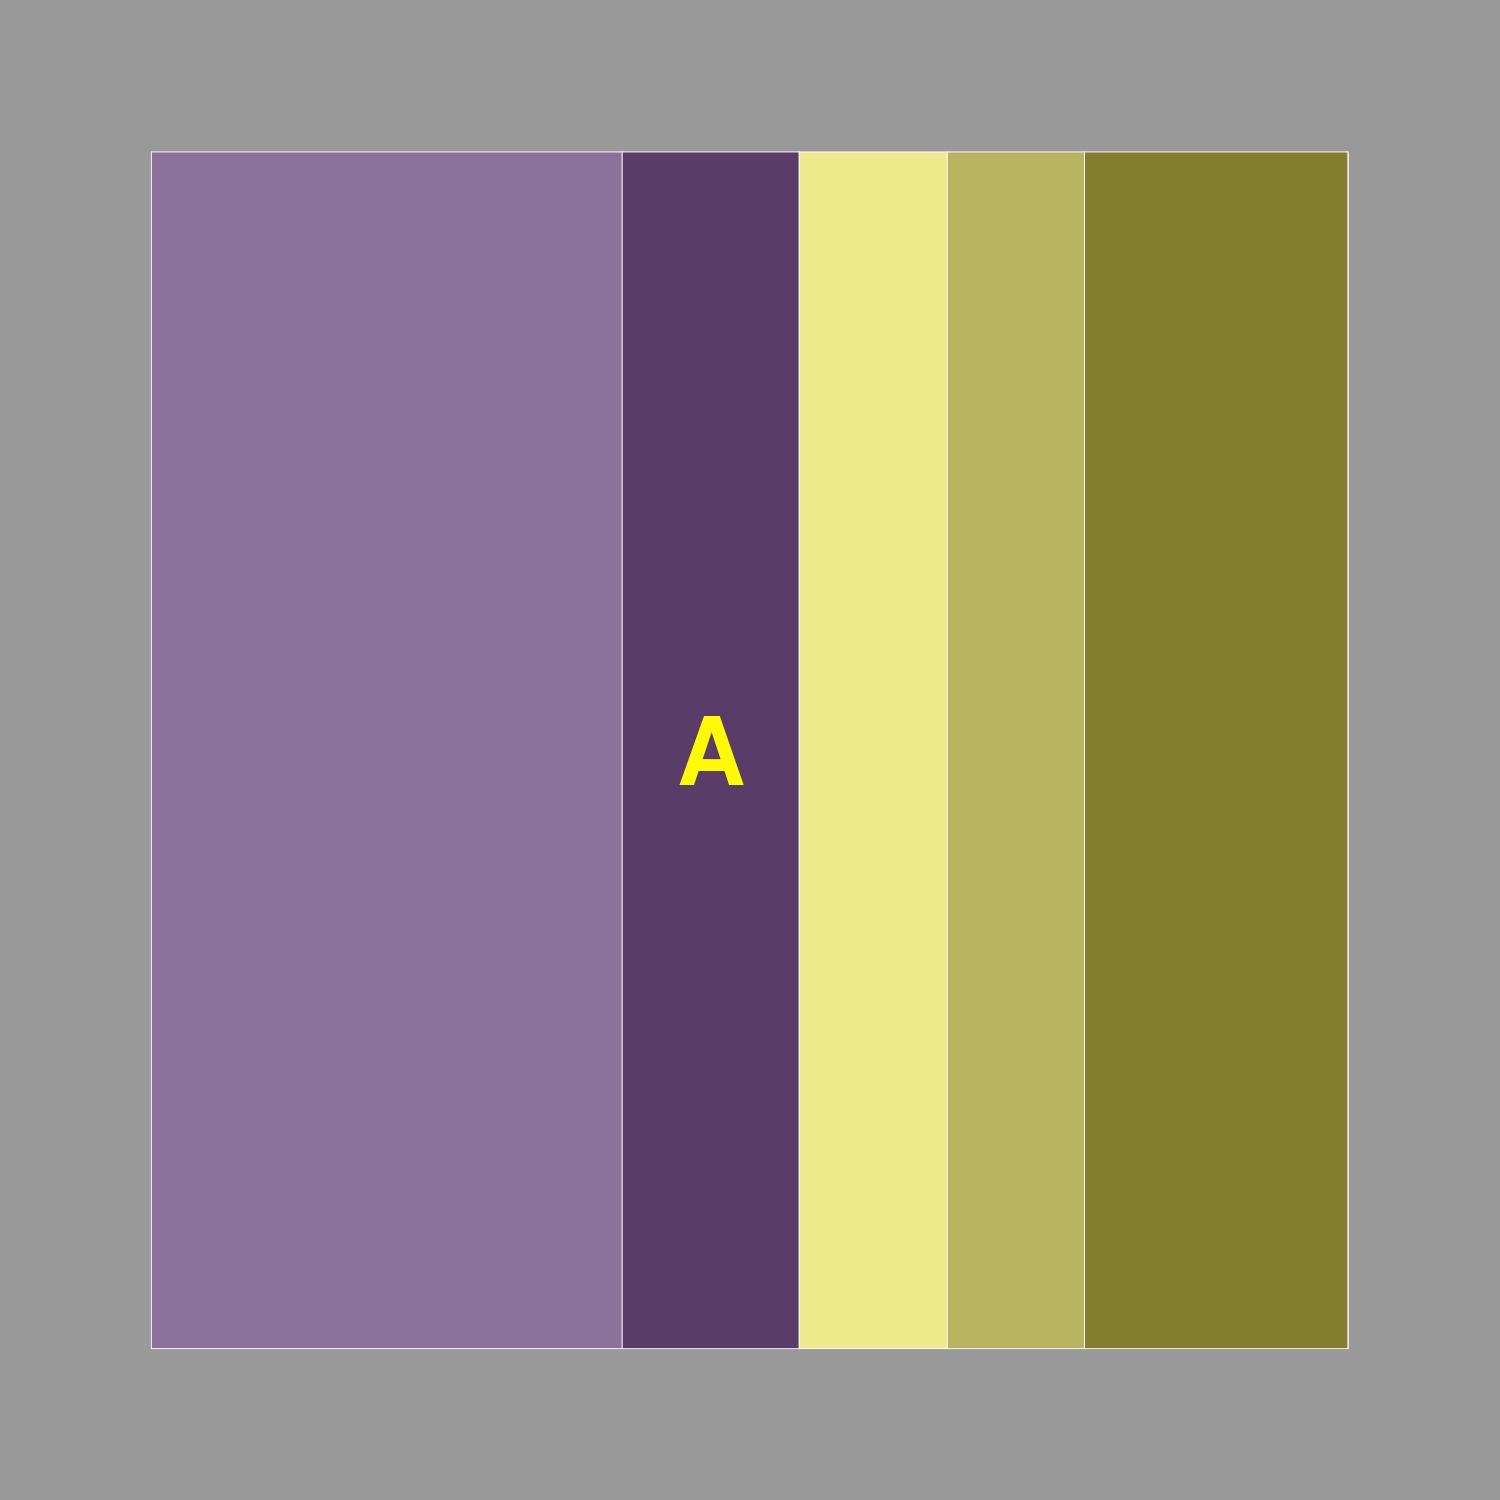
\includegraphics[width=\textwidth]{figure/Oregon-spine_with_frame3.png}
\end{minipage}\hfill
\begin{minipage}{.5\textwidth}
\captionof{figure}{A framed spine plot similar to those shown in the 1874 Statistical Atlas, recreated using modern methods. The chart shows the proportion of church accomodations in Oregon, with the four largest denominationns in the state shown in the center and the unaccommodated population shown in the grey region framing the plot. Participants were asked to estimate the size of the area labeled ``A" relative to the entire chart; the presence of the frame significantly decreases the accuracy of these estimates.~\citep{vanderplasFramedReproducingRevisiting2019}}\label{fig:framedspine}
\end{minipage}

A similar type of study avoids the pitfalls associated with numerical estimation by showing participants multiple charts in sequence, and asking them to evaluate the differences in the charts with respect to the dimension of interest. \citet{shahConceptualLimitationsComprehending1995} required participants to examine the relationship between three variables as shown in several different types of line charts. One set of charts used in the experiment is recreated in \autoref{fig:shahcarpenter}; in the first plot, it is much easier to determine that there is no relationship between pupil size and depression for one level of thyroid activity compared with the second plot.

\begin{knitrout}
\definecolor{shadecolor}{rgb}{0.969, 0.969, 0.969}\color{fgcolor}\begin{figure}
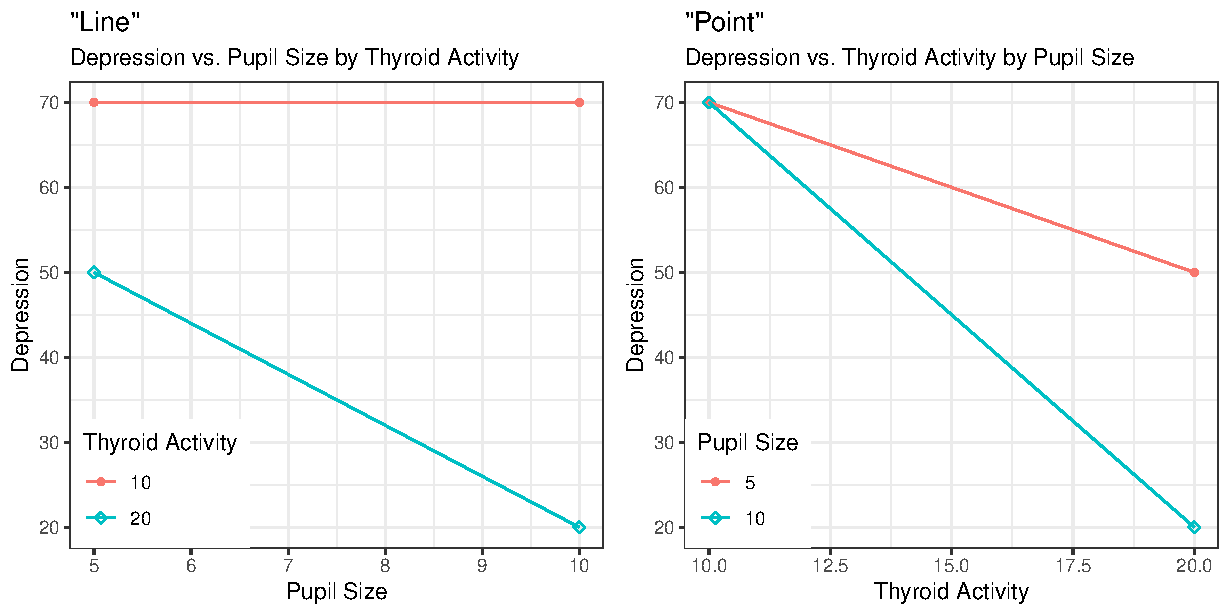
\includegraphics[width=\textwidth]{figure/shahcarpenter-1} \caption[Sample plots from \citet{shahConceptualLimitationsComprehending1995}, showing data where one independent variable (pupil size) has no effect on the y variable (depression) for one value of the second independent variable (thyroid activity)]{Sample plots from \citet{shahConceptualLimitationsComprehending1995}, showing data where one independent variable (pupil size) has no effect on the y variable (depression) for one value of the second independent variable (thyroid activity). The two representations of this data, referred to as line and point, are not equally effective for communicating the joint relationship of the two independent variables. }\label{fig:shahcarpenter}
\end{figure}


\end{knitrout}

In some studies, response time is the main quantity of interest. Participants are provided with a certain chart or stimulus, and the amount of time spent considering the stimulus before answering  are used together with accuracy of the answer to assess the difficulty of the task, under the premise that more difficult or mentally demanding tasks will require more time before a response is generated. \citet{carswellInformationIntegrationObject1987} uses the error rate and response time to determine whether triangular ``object displays" are superior to bar graphs to represent the inputs and outputs of a dynamic system~\citep[see Fig.2 in][for an example of an object display]{carswellInformationIntegrationObject1987}; \citet{leggeEfficiencyGraphicalPerception1989} uses efficiency, a function of time and accuracy, to assess different types of charts. More modern studies may collect both response time and numerical estimation data online, using services such as Amazon Mechanical Turk to conduct usability studies in statistical graphics~\citep{heer2010crowdsourcing}. We have even used direct estimation in combination with online testing to examine very old charts from the 1874 Statistical Atlas~\citep{vanderplasFramedReproducingRevisiting2019}, determining that framed mosaic, spine, and pie charts are sub-optimal graphical representations. \autoref{fig:framedspine} direct estimation used in the experiment; participants entered an estimate of the proportion of the chart represented by the area labeled ``A". It should be noted that some of the other experimental paradigms, such as psychophysics and implicit tests, can also be used in combination with Amazon Turk and other online testing services.

There are limits to what one can test using direct estimation: it is generally preferable to test only very straightforward assessments of the content of a chart or graph, to fit within a simple experimental paradigm. In addition, open-ended estimation tasks elicit certain well-known biases such as the tendency to round to multiples of 5 or 10~\citep{bairdRelativeFrequenciesNumerical1970}. Long-term interaction with a complex graph or chart showing multiple layers of data is generally not ideal within this paradigm, which requires a fixed set of numerical assessments that do not accurately represent how we explore a new, complex graphic. This complexity explain why there are so few studies of rich, complex graphics that may require domain expertise in addition to the ability to read information from a visual display. To approach situations with more complicated graphics, or charts which are known to induce perceptual biases in the participants, it is often more useful to utilize other experimental paradigms that facilitate examination of specific parts of the perceptual process - such as the use of eye tracking to measure attention and motivation, or the use of verbal descriptions to assess more complicated graphs. The next sections cover some of these more nuanced approaches to explicit testing of graphs.

\paragraph{Psychophysics and Signal Detection Theory} % .5 page
Some studies of graphs utilize psychophysics methodology to assess data visualizations. Initially, of course, a significant portion of the research in statistical graphics came from the fields of psychophysics and cognitive psychology~\citep{spenceVisualPsychophysicsSimple1990,teghtsoonian_judgment_1965, lewandowskyPerceptionStatisticalGraphs1989}, but in most cases this was not accompanied by a  use of the methods of psychophysics for experimental testing of charts and graphs. Psychophysical experimental design is focused on whether an effect is detectable, and whether the magnitude of the effect can be accurately estimated. Common methods, such as the method of constant stimuli and the method of adjustment, involve repeatedly presenting a participant with charts and asking them to evaluate the chart on the basis of a particular question of interest. In the method of adjustment, this is done with the control of the participant, who adjusts the stimuli interactively until the effect is just barely noticable; in the method of constant stimuli, the effect size changes randomly from trial to trial to reduce continuity effects. In graphical testing, \citet{hughesJustNoticeableDifferences2001} used the method of constant stimuli to assess the ability to detect a difference in height in 2D or 3D barcharts; \citet{vanderplas_signs_2015} used the method of adjustment to experimentally determine the size of the line-width illusion's distortion of variance perception. Psychophysics methods also seem to be relatively common in studies of map perception, particularly when the goal is to estimate the amount of exaggeration or other corrective distortion necessary for realistic perception of the map~\citep[for an overview of relevant cartography studies, see][]{brandesPresentStatePerceptual1976}.


\paragraph{Thinking Aloud} % .5 page
Another approach to testing graphics is to examine the cognitive processes which occur as a graph is read. Lacking mind-reading devices, the next best option is to ask participants to talk through their thoughts as they read and use a graph in a realistic setting (Concurrent Think Aloud, CTA), or as they recall a graph after the fact (Retrospective Think Aloud, RTA)~\citep{guan_validity_2006}. The think aloud process allows experimenters to examine the use of complex graphics ``in the wild" or at least in situations that are less artificial than the paradigms allowed by numerical estimation and psychophysics methods. Think-aloud studies allow researchers to attempt to measure insight~\citep{northMeasuringVisualizationInsight2006} and reasoning~\citep{dunbar1995scientists} in complex situations such as experimental design, decision making~\citep{normandEffectsCelerationLines2006}, or the process of weather forecasting~\citep{traftonTurningPicturesNumbers2000,kirschenbaum2003comparative}. In forensics, think-aloud studies are known as ``white box" studies, because it is possible to ``see" what a forensic examiner is thinking and why they make a specific conclusion about the evidence~\citep{Ulery7733}. Studies using think-aloud protocols have also examined the process of exploratory data analysis, finding that unexpected results are more likely to be represented in informal terms initially, but that with familiarity language shifts to formal explanations~\citep{trickettDipsyDoodlesStreamingMotions2000,trickett2000blobs}. The think-aloud protocol is also conducive to use with interactive graphics, combined with logging or video recording software which can record the state of the graphics device in parallel with the user's monologue. Studies have also combined think aloud protocols and eye tracking studies with the goal of validating CTA~~\citep{cookeAssessingConcurrentThinkAloud2010} and RTA protocols~\citep{guan_validity_2006} for use with statistical graphics and general usability testing. While the data which results from the think-aloud protocol is typically more qualitative and less quantitative than results produced using other methods, there is significant additional insight into the underlying cognitive processes  affecting visualization which cannot be obtained through other means.

\paragraph{Eye Tracking} % .5 page
Where think-aloud protocols allow insight into the cognitive process, eye tracking facilitates insight into the process of visual attention, providing data on the approximate spatial location of visual focus. The attention-fixation process occurs too quickly to be accurately verbally communicated, but eye-tracking equipment allows experimenters to identify the portions of the chart which require attention and sustained cognitive effort or which attract interest from participants, inferring from gaze and fixation the cognitive processes occurring during graph comprehension. Eye tracking allows researchers to determine that viewers spend relatively little time examining the axes in scatterplots, but significant amounts of time examining the axes in parallel coordinates plots~\citep{netzelComparativeEyetrackingEvaluation2017}, suggesting that the process of reading these two chart types is fundamentally different. Another study leveraged eye tracking to identify features which provide useful information during the graph reading process for several different types of charts~\citep{goldbergComparingInformationGraphics2010}. Eye tracking is a powerful tool when combined with good experimental design: \citet{fabrikantCognitivelyInspiredPerceptually2010a} examined fixations when shown meterological charts before and after users are provided with introductory training about meterology, finding that after training users conclusions were more accurate, response time increased, and fixations were directed to more useful areas of the maps. The use of eye tracking with different source populations also allows researchers to understand how dyslexia~\citep{kimInvestigatingGraphComprehension2014} and graph literacy~\citep{wollercarterCommunicatingDistortingRisks2012,okanHowPeopleLow2016} affect the graph comprehension process, providing better design guidelines for specific target audiences.


% A plot of gaze/fixation would be cool here, esp. in combination with a picture of an eye tracking rig, but I can't find anything that's labeled for reuse that's of sufficient quality...

\paragraph{Combination Experiments}
Many studies use a combination of the explicitly structured graphical tests discussed here. Think-aloud studies are relatively easy to integrate with eye tracking studies, and it is not difficult to add in direct observations or psychophysical evaluation methods as part of the trial design. Psychophysics and direct observation studies are limited by the questions that are asked; eye tracking results only provide information on visual focus; think-aloud results are generally qualitative, but when these techniques are combined, they provide a much more complete picture of the cognitive processes which underlie graphical perception. \citet{ryuExploringCognitiveStrategies2003} used a combination of eye tracking, cognitive tests, direct observation, and think-aloud protocols to examine the integration of information across multiple types of charts, determining that integrating information from multiple parallel coordinates plots is slow, difficult, and inaccurate compared to information integration when a scatterplot or map is presented with a parallel coordinate plot. \citet{zgraggenInvestigatingEffectMultiple2018} also used a combination of think aloud, eye tracking, direct observation, and interactive graphics to examine the impact of exploratory data analysis on multiple testing problems. Many of the attention-mediated, explicitly structured testing methods can also be combined with implicitly structured tests, which we discuss in the next section, to produce a more comprehensive view of the process of graphical perception.



\subsection{Implicit Graphical Tests Using Visual Inference} % 4-5 pages
% This portion of the section will examine the use of visual inference methods. Visual inference quantifies the significance of a visual finding, sidesteps many of the generalizability issues seen in the explicit tests discussed in the previous section, and leverages the natural power of the human visual system. We will also explore the power of visual inference combined with the grammar of graphics, as well as novel uses of visual inference to examine the effect of specific features of the data set.

% Eye tracking and thinking aloud are not always used with explicit graphical tests; they can also be used with implicit tests~\citep{zhaoMindReadingUsing2013}, that is, tests which require the participant to determine the relevant characteristics under examination before evaluating a series of charts using the identified characteristic. Implicit tests provide a convenient way to compare graphical designs, extending statistical inference to a visual domain\citep{bujaStatisticalInferenceExploratory2009}.

Explicit graphical tests, as we have referred to them, are tests where the user is directed to assess a specific feature of a plot or answer a specific question.
That is, the tested hypothesis is explicitly stated, providing the user with cues to the intended purpose and function of the plot and/or the relevant features of the data shown within the plot.
In contrast, in an implicit graphical test, the user must identify both the purpose and function of the plot and use that information to evaluate the plots as shown.
Typically, these tests are structured as visual inference problems, as introduced in \citet{bujaStatisticalInferenceExploratory2009}, though other formulations of implicit tests exist as well~\citep{hasanhodzicHumansPerceiveTemporal2011}.
Explicit tests are typically conducted on plots which have been created to showcase specific structure in the data in order to present results; in contrast, implicit tests are designed to inform exploratory data analysis~\citep[as advocated by][]{tukeyTechnicalToolsStatistics1965} and the iterative model diagnostic process.
During a data exploration (EDA), statisticians typically examine the data using many different plots considering different aspects of the data and selecting only those results which are visually interesting for further exploration.
This raises the question whether the `visually interesting' features in those plots show actual signal and do not arise simply by chance. This question is a direct consequence of our general use of graphics and our definition of `interesting'. Generally speaking, something is `interesting' that does not follow our expectations in some way -- in other words, we conduct an implicit hypothesis test when drawing and looking at charts; `interesting' charts are those which are deemed `significant' according to this implicit hypothesis test. Making this hypothesis test explicit allows for a more formal evaluation of the significance of a visual finding.
In terms of a classical  hypothesis test,  a plot of the data is taking the role of a (visual) test statistic. Null plots are created from data in acordance with the null hypothesis (e.g\ permuted data, if the null hypothesis assumes that there is no non-random relationship between the variables). If the data plot is visibly different from the null plots, i.e.\ can be picked out through visual inspection by an independent evaluator, this counts as evidence against the null hypothesis and once enough evidence is accumulated we would conclude that the null hypothesis has to be rejected and accept that the feature in the data plot is not random.
Formally, a statistical lineup of $m$ visual statistics consists of $m-1$ plots $T(y_0)$ simulated from the model specified by the null hypothesis, and the test statistic $T(y)$ produced by plotting the actual data, which may arise from the alternative hypothesis. \autoref{fig:lineup-demo} demonstrates this process, with the 19 null plots generated by randomizing the values of $y$. The statistical lineup is then evaluated by $K$ independent observers, with the resultant p-value calculated according to the null hypothesis that each of the $m$ visual statistics are equally likely to be selected~\citep{majumderValidationVisualStatistical2013}. The \texttt{nullabor} package contains tools for graphical inference~\citep{nullabor}, including p-value calculations and power calculations for visual inference.

\begin{figure}
% \begin{minipage}{.3\textwidth}
% <<lineup-setup, fig.width = 3, fig.height = 3, out.width = "\\textwidth", include = T, echo = F>>=
% set.seed(4209510)
% x <- jitter(seq(0, 1, length.out = 50))
% y <- rnorm(n = length(x), mean = x, sd = .3)
% y <- (y - min(y))/(max(y) - min(y))
% df <- tibble(x = x, y = y)
% qplot(x = x, y = y) +
%   coord_fixed() +
%   theme(axis.text = element_blank(), axis.title = element_blank()) +
%   ggtitle("Original Data")
% @
% \end{minipage}
% \begin{minipage}[c]{.69\textwidth}
% <<lineup-creation, fig.width = 10, fig.height = 8, out.width = "\\textwidth", include = T, echo = F>>=
% lineup(null_permute("y"), df, pos = 9) %>%
%   ggplot(aes(x = x, y = y)) +
%   geom_point() +
%   facet_wrap(~.sample) +
%   coord_fixed() +
%   theme(axis.text = element_blank(), axis.title = element_blank(), plot.title = element_text(size = 20)) +
%   ggtitle("Plot Lineup")
% @
% \end{minipage}
\begin{minipage}{.3\textwidth}
\begin{knitrout}
\definecolor{shadecolor}{rgb}{0.969, 0.969, 0.969}\color{fgcolor}
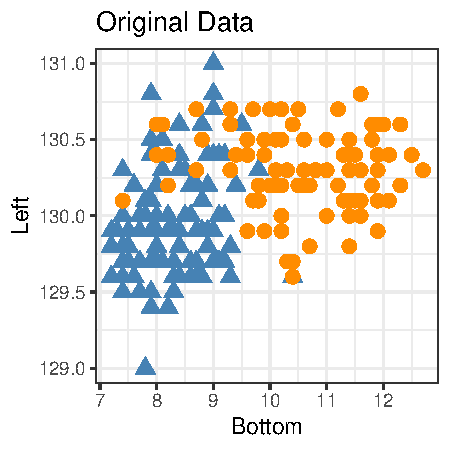
\includegraphics[width=\textwidth]{figure/lineup-setup2-1} 

\end{knitrout}
\end{minipage}
\begin{minipage}[c]{.69\textwidth}
\begin{knitrout}
\definecolor{shadecolor}{rgb}{0.969, 0.969, 0.969}\color{fgcolor}
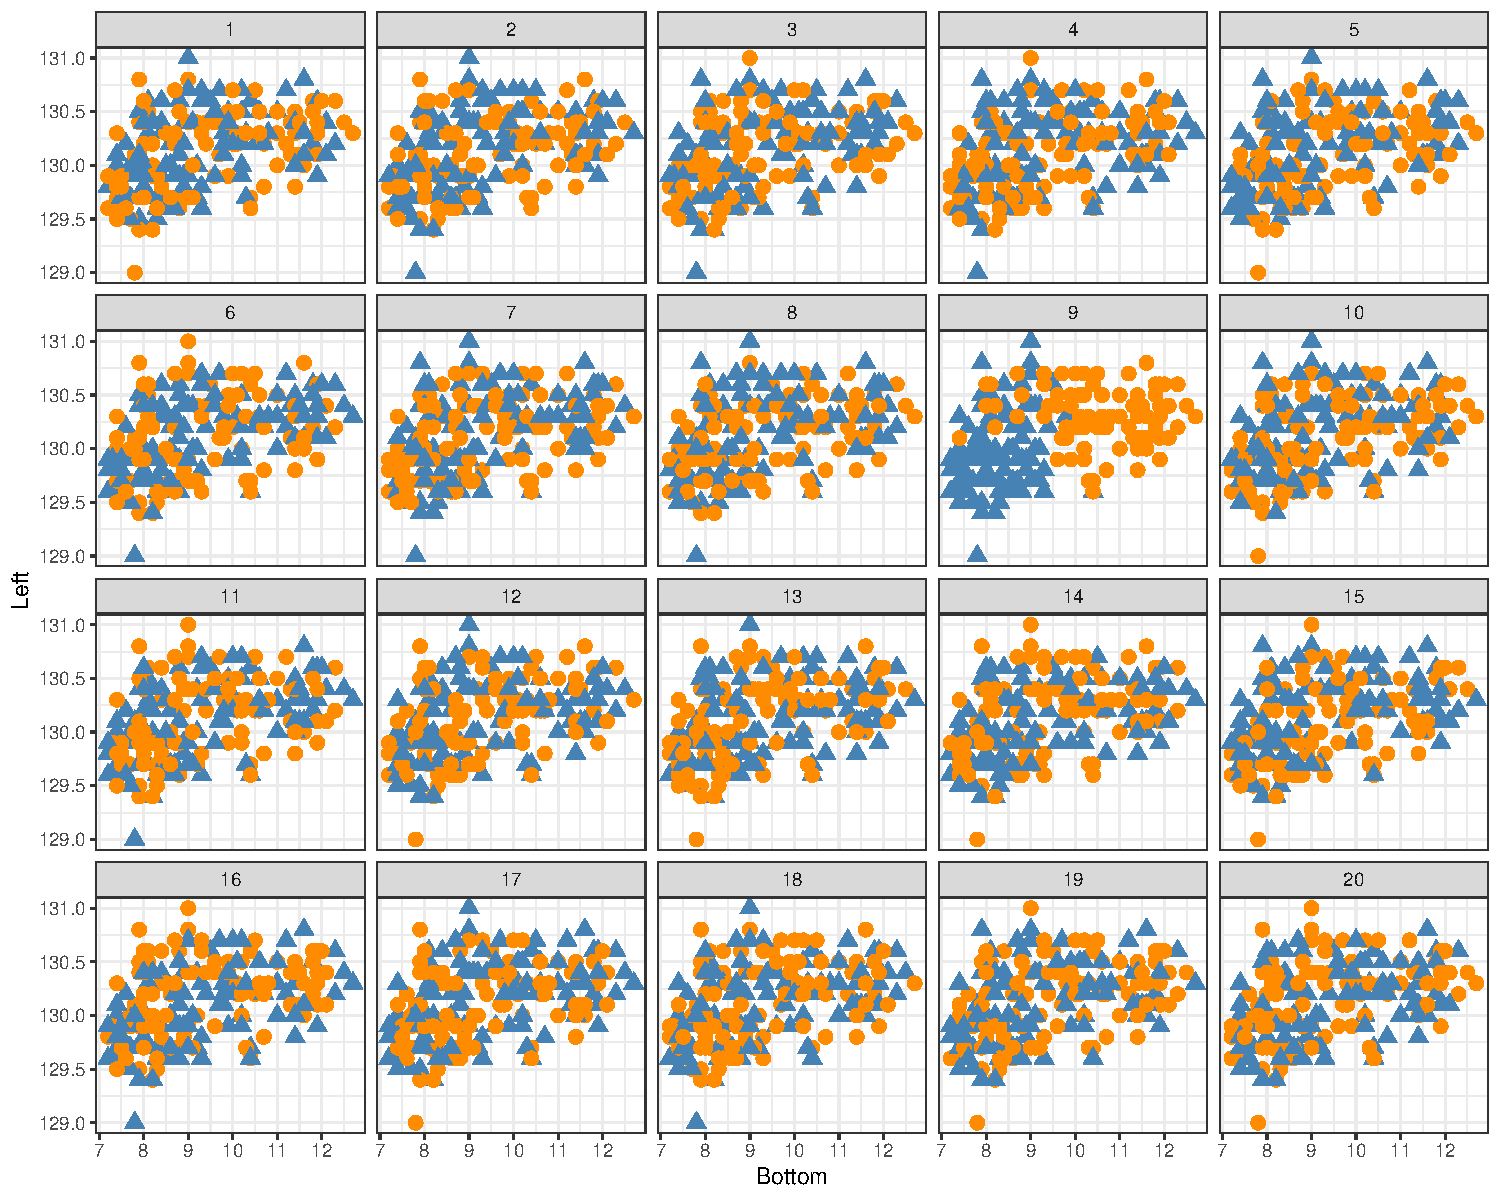
\includegraphics[width=\textwidth]{figure/lineup-creation2-1} 

\end{knitrout}
\end{minipage}
\caption{The original data (left) is embedded into a set of 19 generated under the null hypothesis. A visual hypothesis test is conducted by asking multiple users to select one (or more) plots which are different; a p-value can then be calculated from the answers. In this particular lineup, plot 11 contains the original data; the other plots are generated by randomizing the vector of colour/shape values as in a randomization test.}\label{fig:lineup-demo}
\end{figure}

Implicit graphical tests approach the problem of spurious plot relationships at the level of the data, leveraging the human visual system to conduct a suite of visual tests for features such as outliers, clusters, linear and nonlinear relationships.
The advantage to implicit testing is that lineups do not require a specification of a feature of interest in the testing framework, i.e.\  we do not have to ask questions such as ``which group has a higher proportion of responses".
Much of the historical research of comparing different types of charts has been criticized because the specific question phrasing does not provide readily generalizable results; the lineup protocol removes this obstacle by charging the user with the task of identifying the most different looking plot and thereby selecting the feature with the visually most salient difference compared to the other plots.
%Using visual inference, we simply show a series of plots and depend on the user to identify that one of the plots looks different.
This allows an evaluation of competing plot designs without the complications of potentially steering participants towards a particular outcome by phrasing questions. This leads to a completely data-driven result: if bar charts are indeed better suited for a task than pie charts, the target plot will be selected more frequently when the lineup is presented with bar charts than when the lineup is presented with pie charts.
The real power of the lineup protocol is that when \emph{combined with the grammar of graphics}, we can hold the underlying data and summary statistics constant, isolating the effect of different plot types, coordinate transformations, and aesthetic mappings on our ability to detect effects in the data.

% Might be worth mentioning papers which use visual inference casually (not experimentally) to make a point? Don't want to throw those in with the formal testing papers though...

Statistical lineups have been used experimentally to examine single plot types in many contexts: residual plots in hierarchical linear models~~\citep{loyAreYouNormal2015}, perceived clustering in high-dimensional data~\citep{roychowdhuryUsingVisualStatistical2015}, and spatial clustering in geographical research~\citep{widen2016graphical}. \citet{loyVariationsQQPlots2016} used statistical lineups to evaluate different types of Q-Q plots for assessing violations of normality, determining that the visual tests were generally more powerful than common numerical tests when assessing violations of normality. \citet{beechamMapLineUpsEffects2017} used lineups to assess the effect of spatial autocorrelation when represented using different grid structures, finding that lineups can be used for chloropleth maps if the null plots are generated under models with reasonable spatial autocorrelation models. Other studies have also found that the approach to null model generation is critical. It can be difficult to specify the null data generating model in a way that adequately mimics the data plots, which suggests that visually we are able to identify many more features than those typically tested using standard quantitative hypothesis tests. This implicit testing of many different hypotheses does make null distribution specification challenging, but also highlights the power of visual cognition to detect subtle differences in data.

Typical lineups contain a single target plot, but this is not a requirement. \citet{vanderplasClustersBeatTrend2017} used two targets, each generated from a competing data model: clustering, or linear association. The null plots in this experiment were composed of a mixture of points generated from each of the two data models, ensuring that the two targets were both slightly more extreme than the null plots, but that the null plots and the target plots shared some features. Using this approach, the authors tested the effect of different aesthetics on the selection of each of the two targets, examining the strength of aesthetics such as colour, shape, trend lines, error bands, and 95\% ellipses for highlighting clustering or linear trends in the data. By providing viewers with a choice between data generated by competing models, the two-target lineup approach provides a way to directly examine the visual strength of each model compared to the null and comparing the models directly. For instance, when comparing a model generating clustered data to a model generating data with a linear association between y and x, this protocol establishes that colour and shape aesthetics slightly increase the likelihood that the cluster target plot is selected, while a trend line aesthetic slightly increases the probability that the linear relationship target plot will be selected. More broadly, \citet{vanderplasClustersBeatTrend2017} shows that the aesthetics used in a plot can significantly impact the perceived relationship between variables.

In the ten years since the introduction of the lineup protocol, many studies have leveraged the grammar of graphics to ensure that the underlying data mapping remains the same while manipulating the geometric representation of the data and overall visual appearance of the plot. Combining the conclusions from both implicit lineup tests and the explicit tests described in the previous section, what can we say about best graphical practices, beyond ``pie charts are awful"?

\section{CURRENT BEST GRAPHICAL PRACTICE} % 3.5 pages
% The previous section discussed methods for testing hypotheses about best graphical practice, but can we draw any conclusions about what current best graphical practice is? This section will summarize the conclusions from the testing methods, organized by topic. Potential topics include bar charts, the selection of aesthetics such as colour, shape, and shading, double encoding, and polar coordinate systems.

All of the user testing in the world cannot identify the ``best" possible graphic -- we can instead only experimentally assess which graphical designs are better for a specific purpose. This can lead to a rather fragmented approach when describing ``best practice", and so in order to avoid this, we will examine graphical practice using the principle of ``First, do no harm" from the Hippocratic oath.

\subsection{Cognitive Principles}

A useful starting point is to apply Gestalt principles of visual perception~\citep{gestalt1,gestalt2}, such as proximity, similarity, common region, common fate, continuity, and closure, to data plots. These principles are useful because good graphics take advantage of the human visual system's ability to process large amounts of visual information with relatively little effort. Understanding the principles which underlie this processing allows us to create charts which require less cognitive effort to read, freeing us to think about the content, rather than the form of the chart.

\subsubsection{Proximity}

The principle is `objects or shapes that are close to one another appear to form groups'. For plot design, proximity is used to place items to compare close together, and less important comparisons further apart. Figure \ref{fig:proximity} illustrates this principle when using facetting in a plot, using data on tuberculosis (TB) incidence in Australia in 2012. When plots are {\em facetted by age}, it means gender is easier to compare. We  learn that females more than males are detected to have TB in their early 20s, but in the aging population, males more commonly are detected with TB. Conversely, when plots are {\em facetted by gender}, the distribution of age is easier to examine. We  learn that the age distribution of TB incidence for females skews heavily towards younger women. For males, TB incidence is more uniform across ages because there are high counts at young, old and middle age categories. Effectively utilizing proximity in organising plots, makes a huge difference in ease of information communication.



\begin{figure}
\begin{minipage}{.345\textwidth}
\begin{knitrout}
\definecolor{shadecolor}{rgb}{0.969, 0.969, 0.969}\color{fgcolor}\begin{kframe}
\begin{alltt}
\hlcom{# gender in age}
\hlkwd{ggplot}\hlstd{(tb_au_12,}
       \hlkwd{aes}\hlstd{(}\hlkwc{x} \hlstd{= gender,}
           \hlkwc{y} \hlstd{= count,}
           \hlkwc{fill} \hlstd{= gender))} \hlopt{+}
  \hlkwd{geom_bar}\hlstd{(}\hlkwc{stat} \hlstd{=} \hlstr{"identity"}\hlstd{)} \hlopt{+}
  \hlkwd{facet_grid}\hlstd{(}\hlopt{~} \hlstd{age)}
\end{alltt}
\end{kframe}
\end{knitrout}
\end{minipage}\hfill
\begin{minipage}{.60\textwidth}
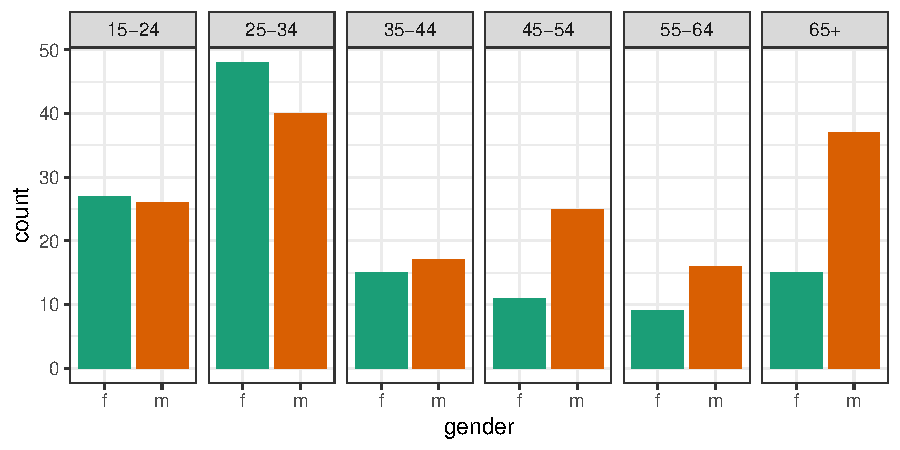
\includegraphics[width=.99\textwidth]{figure/tb-setup-1}
\end{minipage}\\
\begin{minipage}{.345\textwidth}
\begin{knitrout}
\definecolor{shadecolor}{rgb}{0.969, 0.969, 0.969}\color{fgcolor}\begin{kframe}
\begin{alltt}
\hlcom{# age in gender}
\hlkwd{ggplot}\hlstd{(tb_au_12,}
       \hlkwd{aes}\hlstd{(}\hlkwc{x} \hlstd{= age,}
           \hlkwc{y} \hlstd{= count,}
           \hlkwc{fill} \hlstd{= age))} \hlopt{+}
  \hlkwd{geom_bar}\hlstd{(}\hlkwc{stat} \hlstd{=} \hlstr{"identity"}\hlstd{)} \hlopt{+}
  \hlkwd{facet_grid}\hlstd{(}\hlopt{~} \hlstd{gender)}
\end{alltt}
\end{kframe}
\end{knitrout}
\end{minipage}\hfill
\begin{minipage}{.60\textwidth}
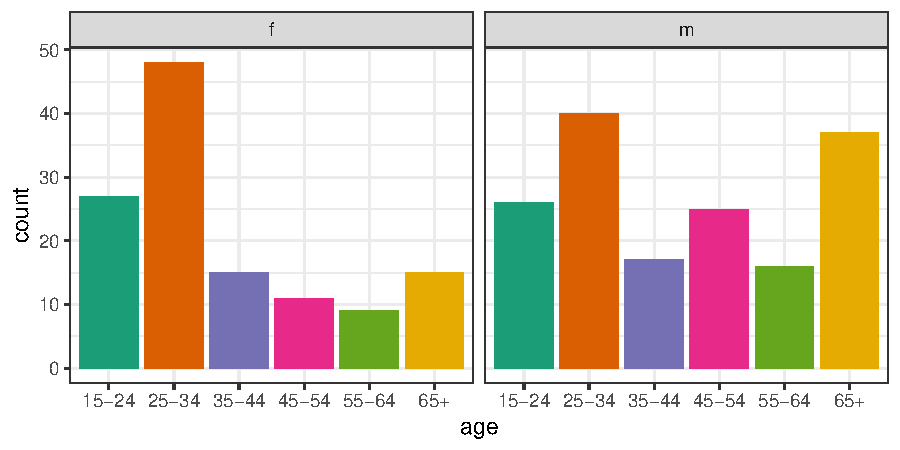
\includegraphics[width=.99\textwidth]{figure/tb-setup-2}
\end{minipage}\\
\caption{Two different arrangements of the same data, to illustrate how the proximity of elements makes a question easier to answer. }\label{fig:proximity}
\end{figure}
\subsubsection{Similarity}
The gestalt principle of similarity suggests that we group things which have similar appearance and exclude objects which have a different appearance. In charts, this principle is often leveraged by colouring points or bars according to a categorical variable, or by using points of different shapes to represent different categories. \citet{vanderplasClustersBeatTrend2017} showed that the addition of colour and shape to a scatterplot increases the likelihood that individuals will perceive clustered groups of points. In \autoref{fig:proximity}, the colouring of bars allows us to easily see that the similarly coloured rectangles represent the same group of people, even though the bars are separated by facets and other groups. % I don't want to bother with another plot for similarity if we can avoid it

\subsubsection{Common Region}
The gestalt principle of common region suggests that elements contained within a common region belong together. Common region helps us to easily read small multiple plots, because the graphical elements of each small plot are grouped into a single entity that can be examined on its own. In addition, confidence bands and bounding ellipses also activate this gestalt principle by grouping points within the boundaries together~~\citep{vanderplasClustersBeatTrend2017}, highlighting the presence of outliers which do not belong to the main group.

\subsubsection{Common fate}
The gestalt principle of common fate describes the tendency to group objects which are moving together in the same direction and at the same speed together. Common fate is certainly active in animated plots which use fading or transitions over time, but even in static plots, continuity can be activated when multiple time series plots are shown together. Figure \ref{fig:commonfate} shows an example. Four examples are displayed as overlaid time series (top), and another four are shown as scatterplots (bottom). In the time series, plot 4 is likely perceived as having stronger association than plot 3, due to the lines moving roughly in a similar pattern. Strong negative association is not easily detected from overlaid line plots, but is easily seen in a scatterplot~\citep{tomasetti}. If negative association is suspected, either using a scatterplot, or inverting one series are suggested.

\begin{knitrout}
\definecolor{shadecolor}{rgb}{0.969, 0.969, 0.969}\color{fgcolor}\begin{figure}
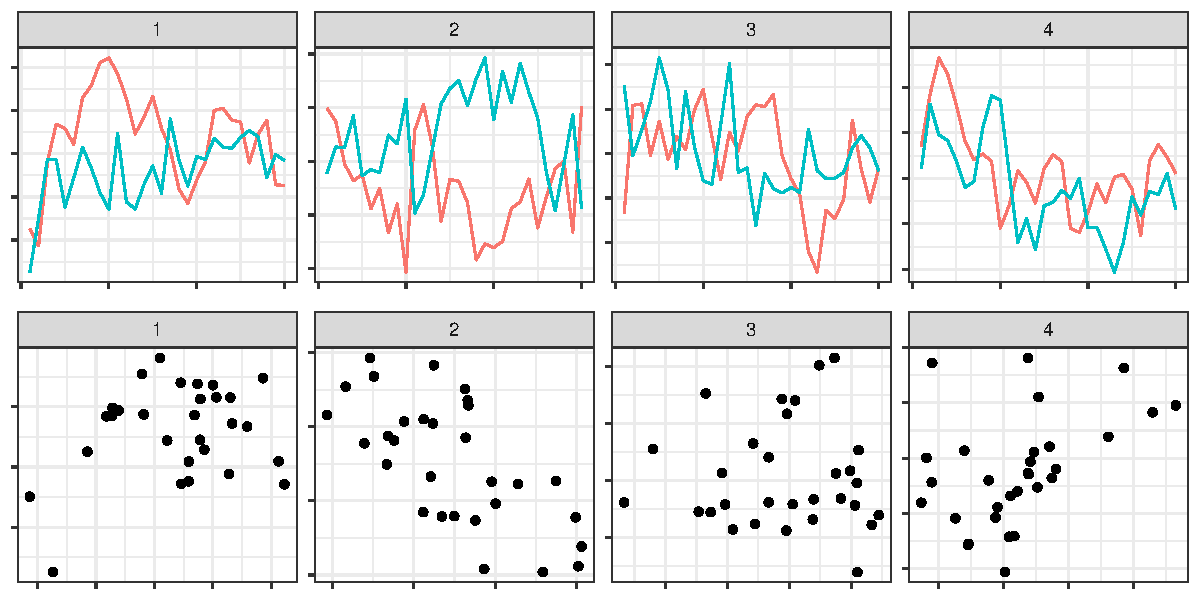
\includegraphics[width=\textwidth]{figure/commonfate-1} \caption[Four examples of pairs of time series displayed as line plots (top) and scatterplots (bottom)]{Four examples of pairs of time series displayed as line plots (top) and scatterplots (bottom). Perception of correlation in overlaid line plots is an example where common fate may dominate. In these four examples of line plots, viewers will likely say that plot 4 has the most similar series, but it is actually plot 2, with strong negative correlation between the two series. A scatterplot clearly shows the negative association.}\label{fig:commonfate}
\end{figure}


\end{knitrout}
% \begin{figure}
% 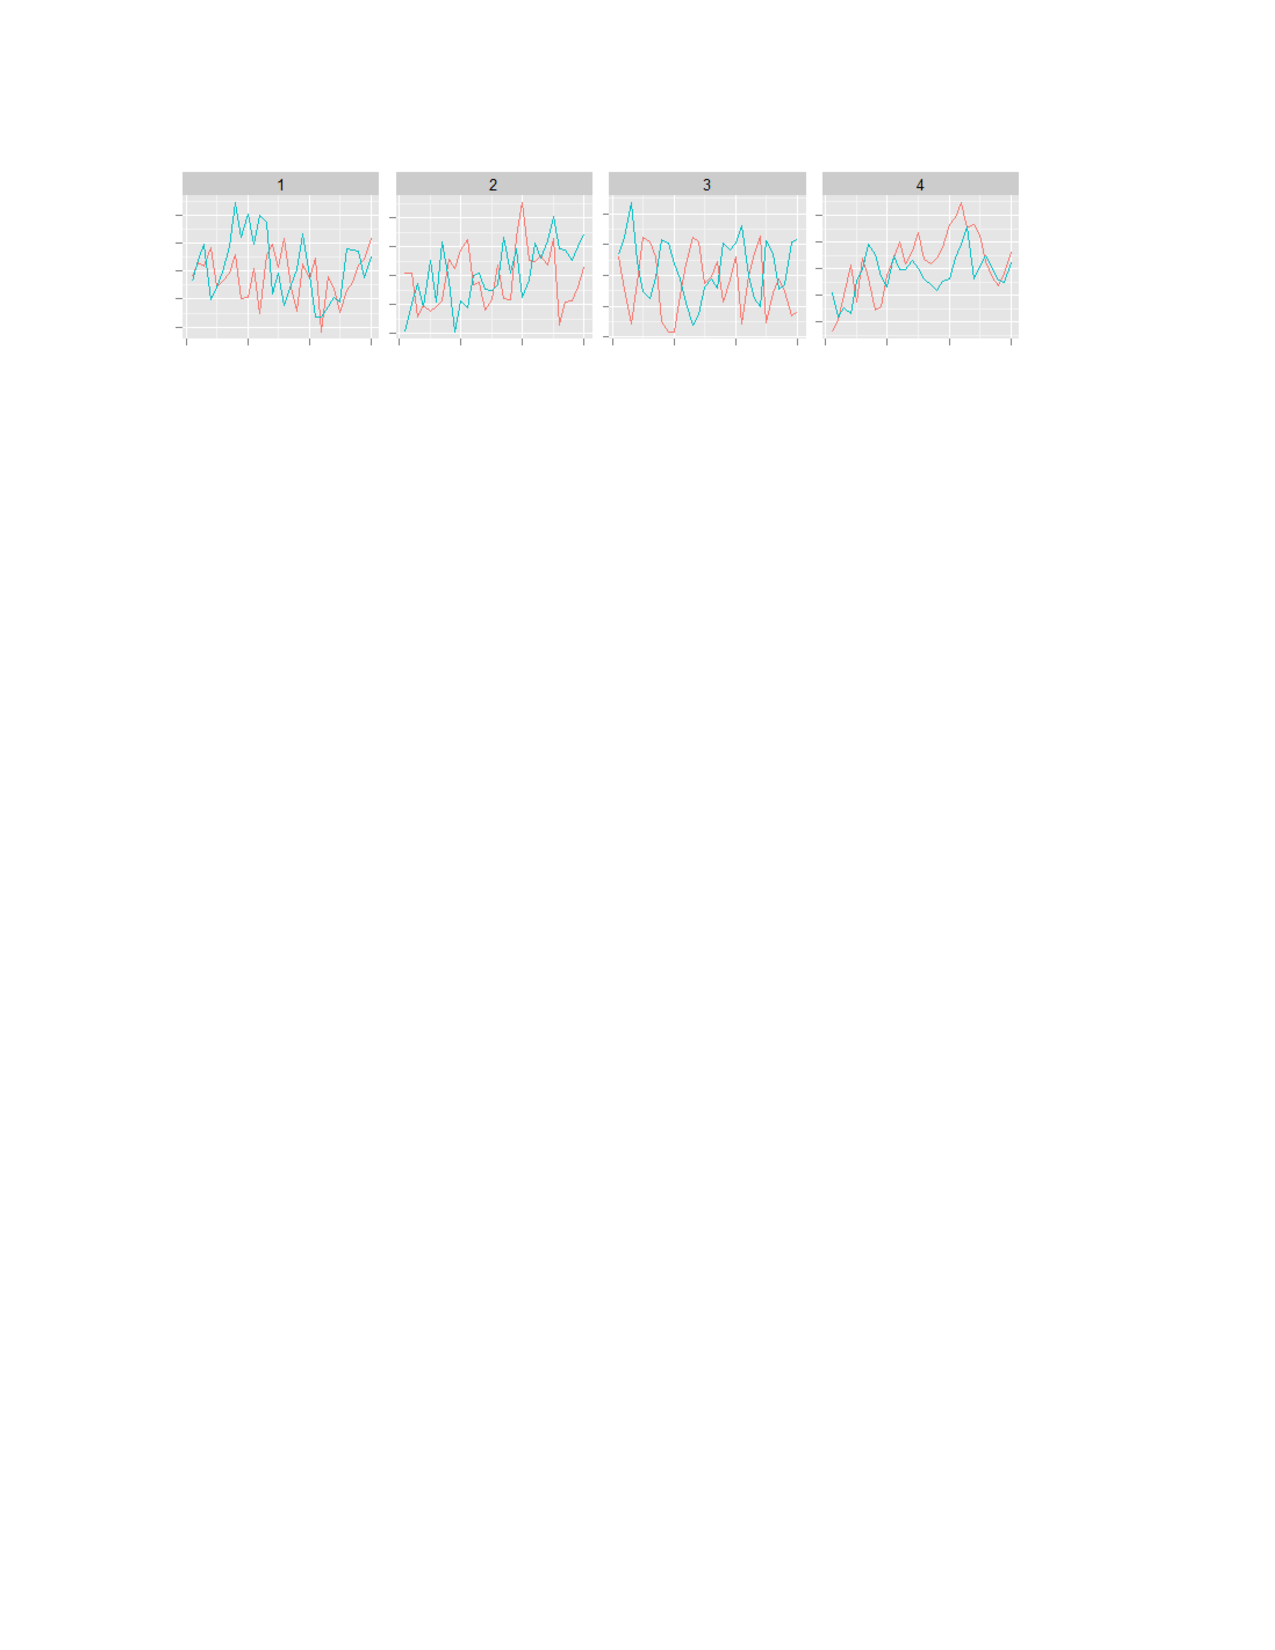
\includegraphics[width=.80\textwidth]{figure/common_fate1.pdf}
% 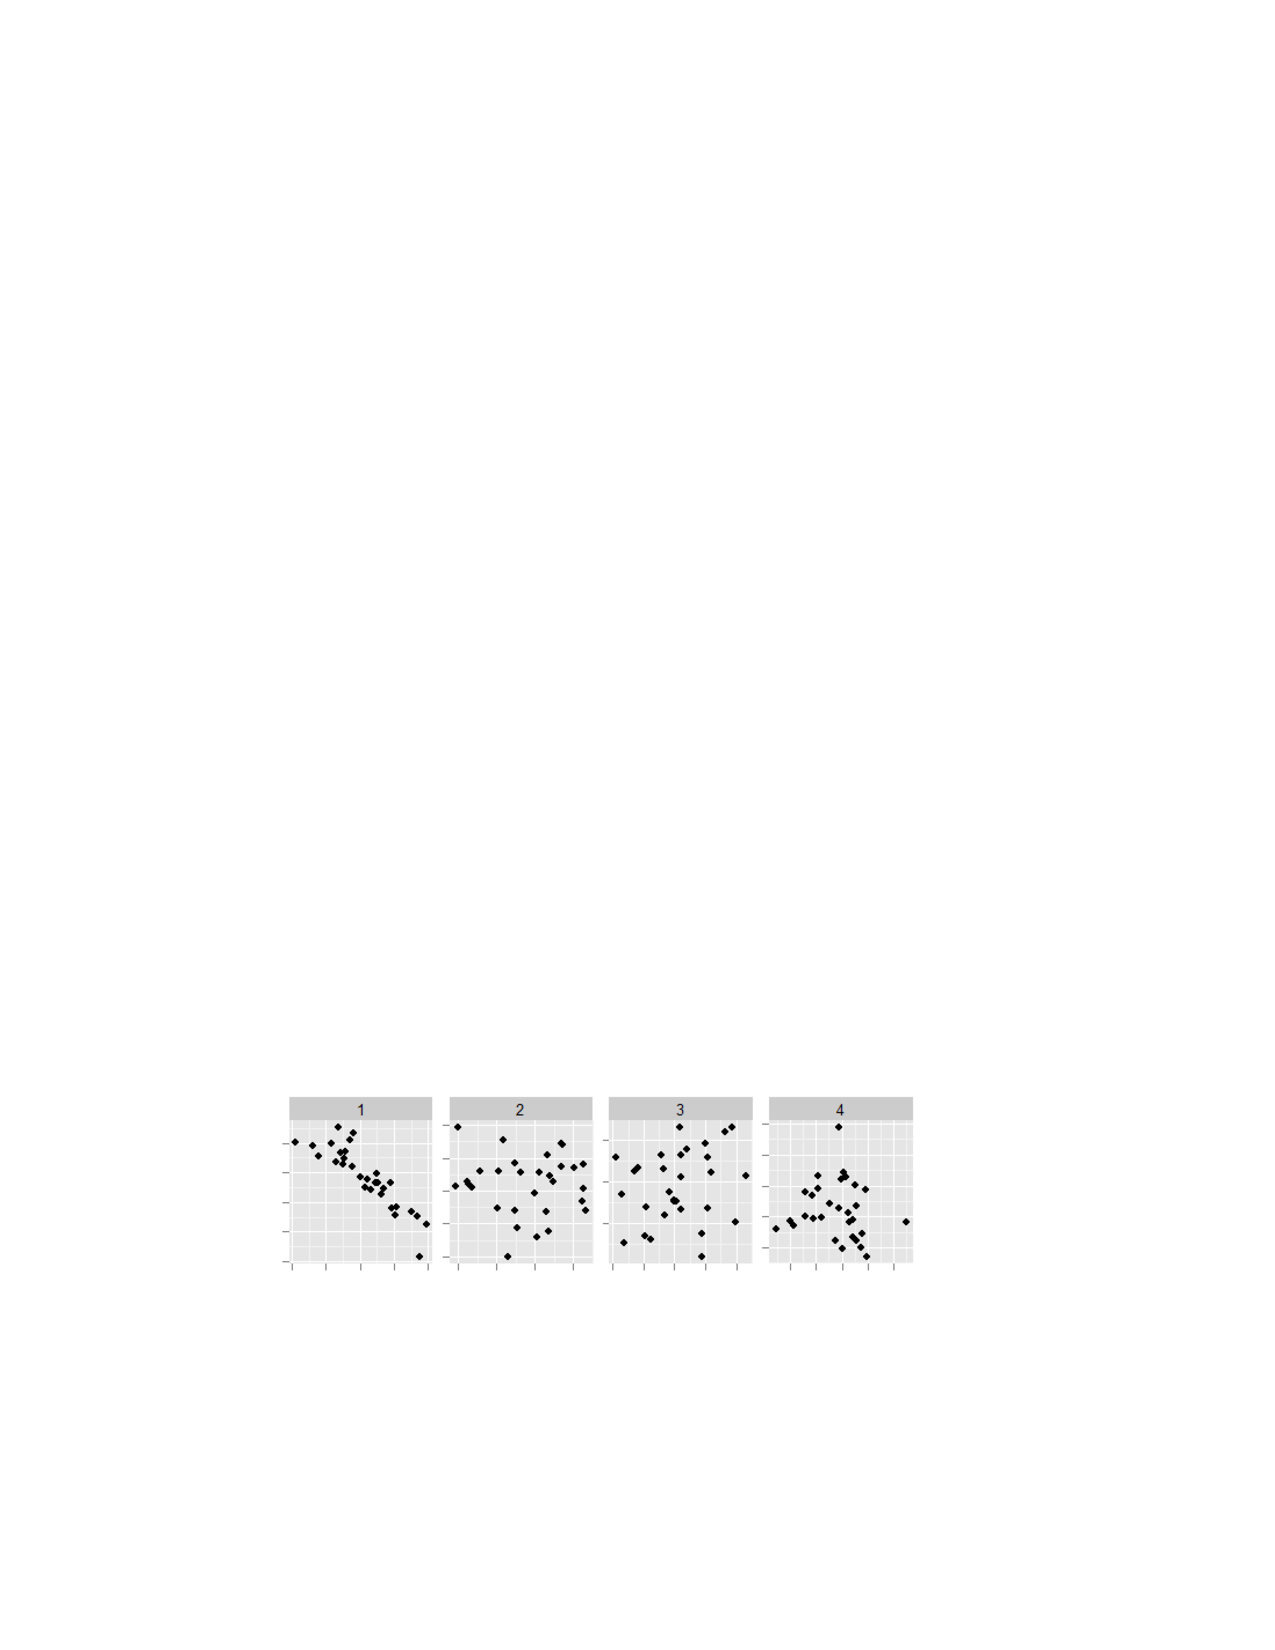
\includegraphics[width=.80\textwidth]{figure/common_fate2.pdf}
% \caption{Four examples of pairs of time series displayed as line plots (top) and scatterplots (bottom). Perception of correlation in overlaid line plots is an example where common fate may dominate. In these four examples of line plots, viewers will likely say that plot 4 has the most similar series, but it is actually plot 3, with strong negative correlation between the two series. A scatterplot clearly shows the negative association (plot 1).}\label{fig:commonfate}
% \end{figure}

%Time series example: positive correlation between two curves as opposed to negative correlation. Plot the two as a scatterplot to communicate correlation, or reverse the sign of one series to check. Refer to Nathaniel Tomasetti's honours thesis? Double axes

Overlaying a few time series on a common scale is one way to activate the heuristic of common fate, but this does not scale well to larger numbers of simultaneous measurements. \citet{javedGraphicalPerceptionMultiple2010a} provide experimental evidence that small multiples are better than other alternatives when there are many simultaneous time series to display and the series cover a large visual span.


\subsubsection{Working Memory}
Another cognitive limitation that affects plot comprehension is the limit on working memory. Typically, working memory is limited to approximately 7 (plus or minus 2) items, or `chunks'. In practice, this means that categorical scales with more than 7 categories decrease readability, increase comprehension time, and require significant attentional resources, because it is not possible to hold the legend mapping in working memory.

\subsubsection{Change blindness}
Not all information is stored in memory (working or long-term) as it is represented. \citet{simonsChangeBlindness1997} suggests that the vivid details available to us instantaneously when examining the world fade quickly, and are replaced with broad semantic descriptions or less meaningful cognitive representations of a scene. As a result of this compression, it is difficult to identify changes between similar scenes. This phenomenon, known as change blindness, affects both static and interactive plots. In static plots, it can be difficult to compare between different small multiples or facets, because the content of the plots are not reliably represented in working memory when switching attention between them. In animated plots, it is important to use transition effects to connect successive frames of the animation: this reduces change blindness and also activates the gestalt principle of common fate, allowing us to quickly identify groups of objects which are transitioning in the same direction.

\subsubsection{Ease of Comparisons}
Much of the psychophysics research on statistical charts examines the accuracy of comparisons and quantitative evaluations made during the process of understanding a plot. This research can be distilled into a hierarchy of comparisons (based primarily on~\citep{cleveland_graphical_1984, cleveland_graphical_1985, shah_cambridge_2005, lewandowskyPerceptionStatisticalGraphs1989}, ranking tasks by their accuracy and difficulty as follows (roughly equivalent tasks are listed together):
\begin{enumerate}
\item Position (common scale)
\item Position (non-aligned scale)
\item Length, Direction, Angle, Slope
\item Area
\item Volume, Density, Curvature
\item Shading, Colour Saturation, Colour Hue
\item Discriminable Shape
\item Indiscriminable Shape
\end{enumerate}

Examples of these charts are shown in \autoref{fig:comparison-ranking}.

\begin{knitrout}
\definecolor{shadecolor}{rgb}{0.969, 0.969, 0.969}\color{fgcolor}\begin{figure}
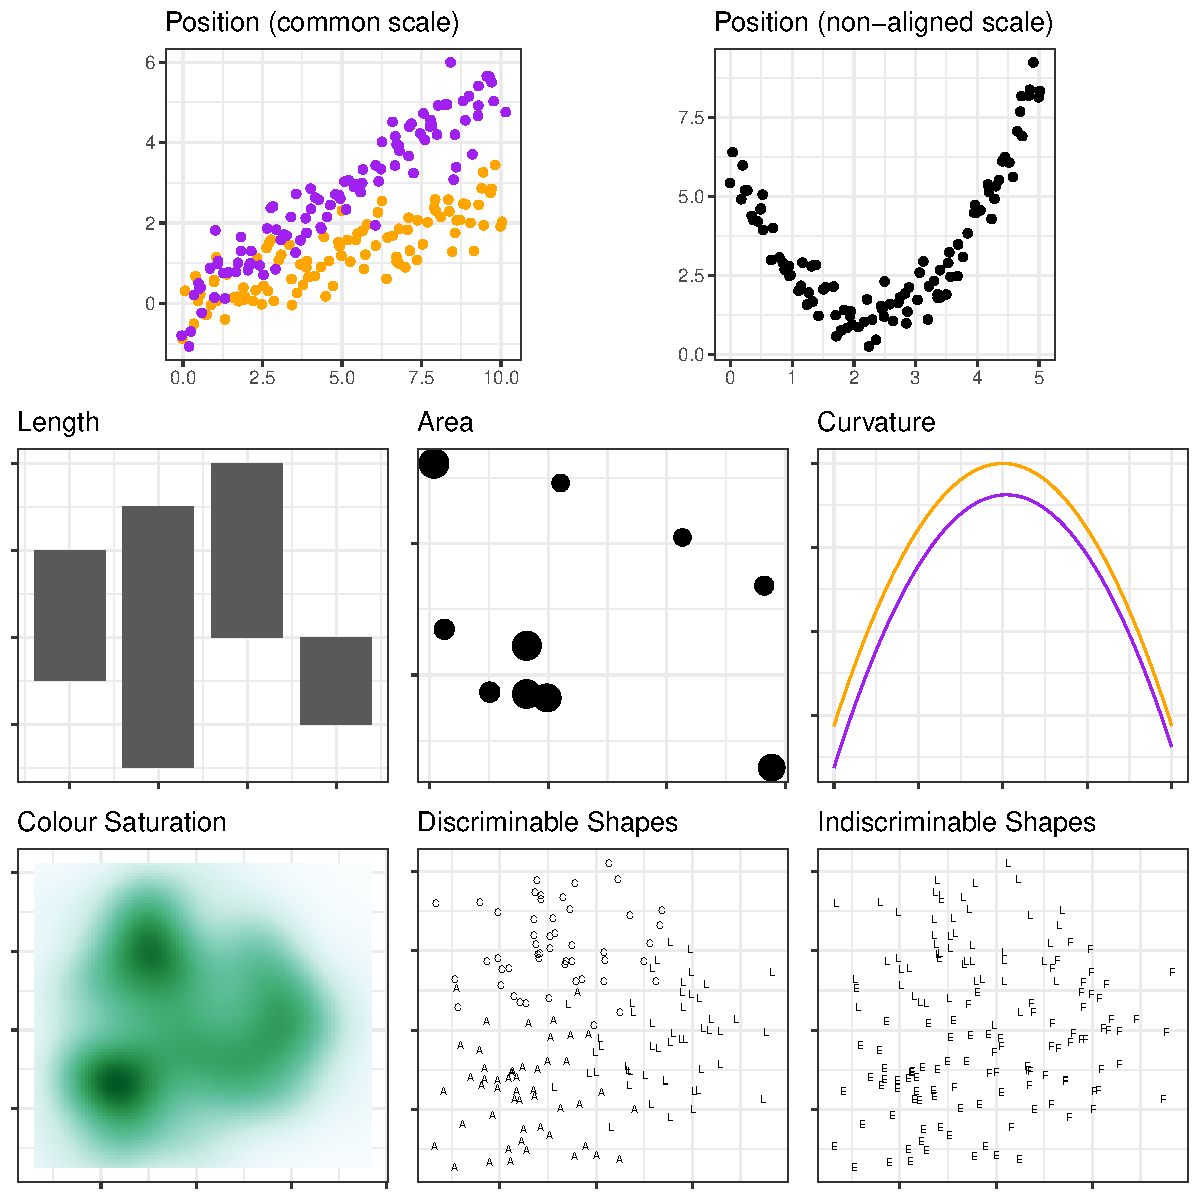
\includegraphics[width=\textwidth]{figure/comparison-ranking-1} \caption[Examples of comparisons, by difficulty]{Examples of comparisons, by difficulty. The first plot shows two sets of points plotted on a common scale; it is easy to compare the relative trajectories of the two lines. The second plot shows another set of points which could be compared to the points in the first plot, however, because the scales are not common between the two, accurate comparisons are more difficult. In the third plot, the rectangles must be compared by length, because they are do not start or end at the same point. In the fourth plot, points are sized based on another variable, requiring comparisons of area; these comparisons are harder to make with numerical accuracy. The fifth plot shows two curves which are not completely parallel, requiring us to make a comparison of curvature; in addition, note that the difference between the two curves is hard to perceive accurately \citep{vanderplas_signs_2015}. The sixth plot shows two-dimensional density using the fill of the tiles; it is possible to make ordered comparisons here but much more difficult to estimate numerical values from the plot even when a legend is provided. The seventh and eighth plots show the same data as the sixth plot, but using discriminable shapes and indiscriminable shapes respectively. Discriminable shapes have different features, while indiscriminable shapes tend to have the same features and require more cognitive effort to separate the clusters.}\label{fig:comparison-ranking}
\end{figure}


\end{knitrout}

This ranking of cognitive tasks provides some consistent guidance for chart design: if the same data can be represented in a way that allows the user to make a comparison more accurately (based on the hierarchy), then that design is preferrable. Thus, this hierarchy indicates that in most cases, it is better to use a stacked bar chart than the equivalent polar-coordinate pie chart, because a stacked bar chart requires evaluation of length, while a pie chart requires area comparisons. If information can be shown on an $x$ or $y$ axis rather than using color (saturation, hue, or shading), it will be easier to make numerical comparisons - we can generally order information based on color, but estimation of numerical quantities is much less precise using color than position. While the hierarchy of graphical comparisons provides some guidance, there are other design choices that can be informed by experimental research in a less systematic way.

\subsection{Chart Design}

\citet{vanderplasClustersBeatTrend2017} provides compelling evidence that the aesthetics used in a chart can significantly affect how plots of the same data are read, and explained these differences relative to the gestalt heuristics activated by each combination of aesthetics. The use of redundant aesthetics which activate the same gestalt principles (such as colour and shape in a scatterplot, which both activate similarity) results in higher identification of corresponding data features. In addition, dual-encoding increases the accessibility of a chart to individuals who have impaired colour vision or perceptual processing (e.g. dyslexia, dysgraphia). This experimental evidence directly contradicts the guidelines popularized by Tufte~\citeyear{tufte}, which suggest the elimination of any feature which is not dedicated to representing the core data, including redundant encoding and other unnecessary graphical elements.

\subsubsection{Colour}
While historically there were constraints on the use of colour in graphics due to technological limitations and the economics of printing, these restrictions have evaporated with the advent of computer-generated graphics, relatively inexpensive colour printing, and an increasing tendency to share charts and graphs digitally instead of in print. Colour can encode categorical and continuous variables, and when used effectively, provides a nearly effortless way to group plot elements using a medium that does not require conscious attention. Unfortunately, while there are many ways to use colour correctly in a plot, there are generally even more ways to use it incorrectly.

Colour scales should be chosen to best match the data values and the plot type: if the goal is to show magnitude, a univariate colour scheme is typically preferrable, while a double-ended colour scale is typically more effective when showing data which differs in sign and magnitude. Where possible, colour scales should use a minimal number of hues, varying intensity or lightness of the colour to show magnitude, and transitioning through neutral colours (white, light yellow) when utilizing a gradient. \autoref{fig:colour-schemes} shows an example of perceptually suboptimal, good, and colourblind accessible diverging colour schemes. Cognitive load can also be reduced by selecting colours which have cultural associations that match the data display, such as the use of blue for men and red (or pink) for women, or the use of blue for cold temperatures and red/orange for warm temperatures.

\begin{knitrout}
\definecolor{shadecolor}{rgb}{0.969, 0.969, 0.969}\color{fgcolor}\begin{figure}
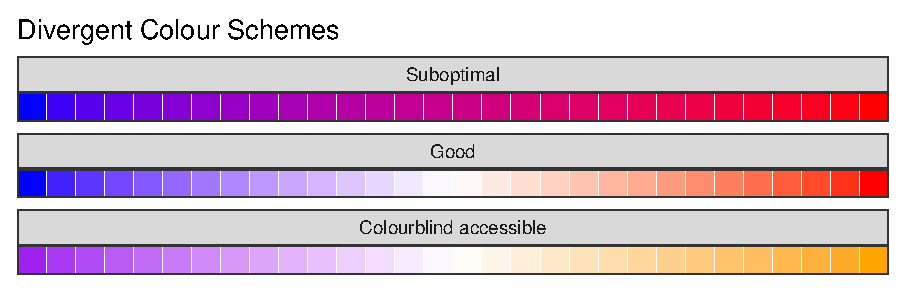
\includegraphics[width=\textwidth]{figure/colour-schemes-1} \caption[Examples of diverging colour schemes which are perceptually suboptimal (no transition through a neutral colour), good, and colourblind accessible]{Examples of diverging colour schemes which are perceptually suboptimal (no transition through a neutral colour), good, and colourblind accessible. The purple - orange gradient through white is distinguishable by individuals with any type of colour deficiency affecting one of the three cones in the retina.}\label{fig:colour-schemes}
\end{figure}


\end{knitrout}

It is also important to consider the human perceptual system, which does not perceive hues uniformly: we can distinguish more shades of green than any other hue, and fewer shades of yellow, so green univariate colour schemes will provide finer discriminability than other colours because the human perceptual system evolved to work in the natural world where shades of green are plentiful. \autoref{fig:perceptual-colourspace} shows the CIE 1931 colour space which maps the wavelength of a colour to a physologically based perceptual space; a significant portion of the colour space is dedicated to greens and blues, while much smaller regions are dedicated to violet, red, orange, and yellow colours. This unevenness in mapping colour is one reason that the multi-hued rainbow colour scheme is suboptimal -- the distance between points in a given colour space may not be the same as the distance between points in perceptual space~\citep{lightEndRainbowColor2004,wakitaSmartColorDisambiguationFramework2005,borlandRainbowColorMap2007}. As a result of the uneven mapping between colour space and perceptual space, multi-hued colour schemes are not recommended.

\begin{minipage}{.4\textwidth}
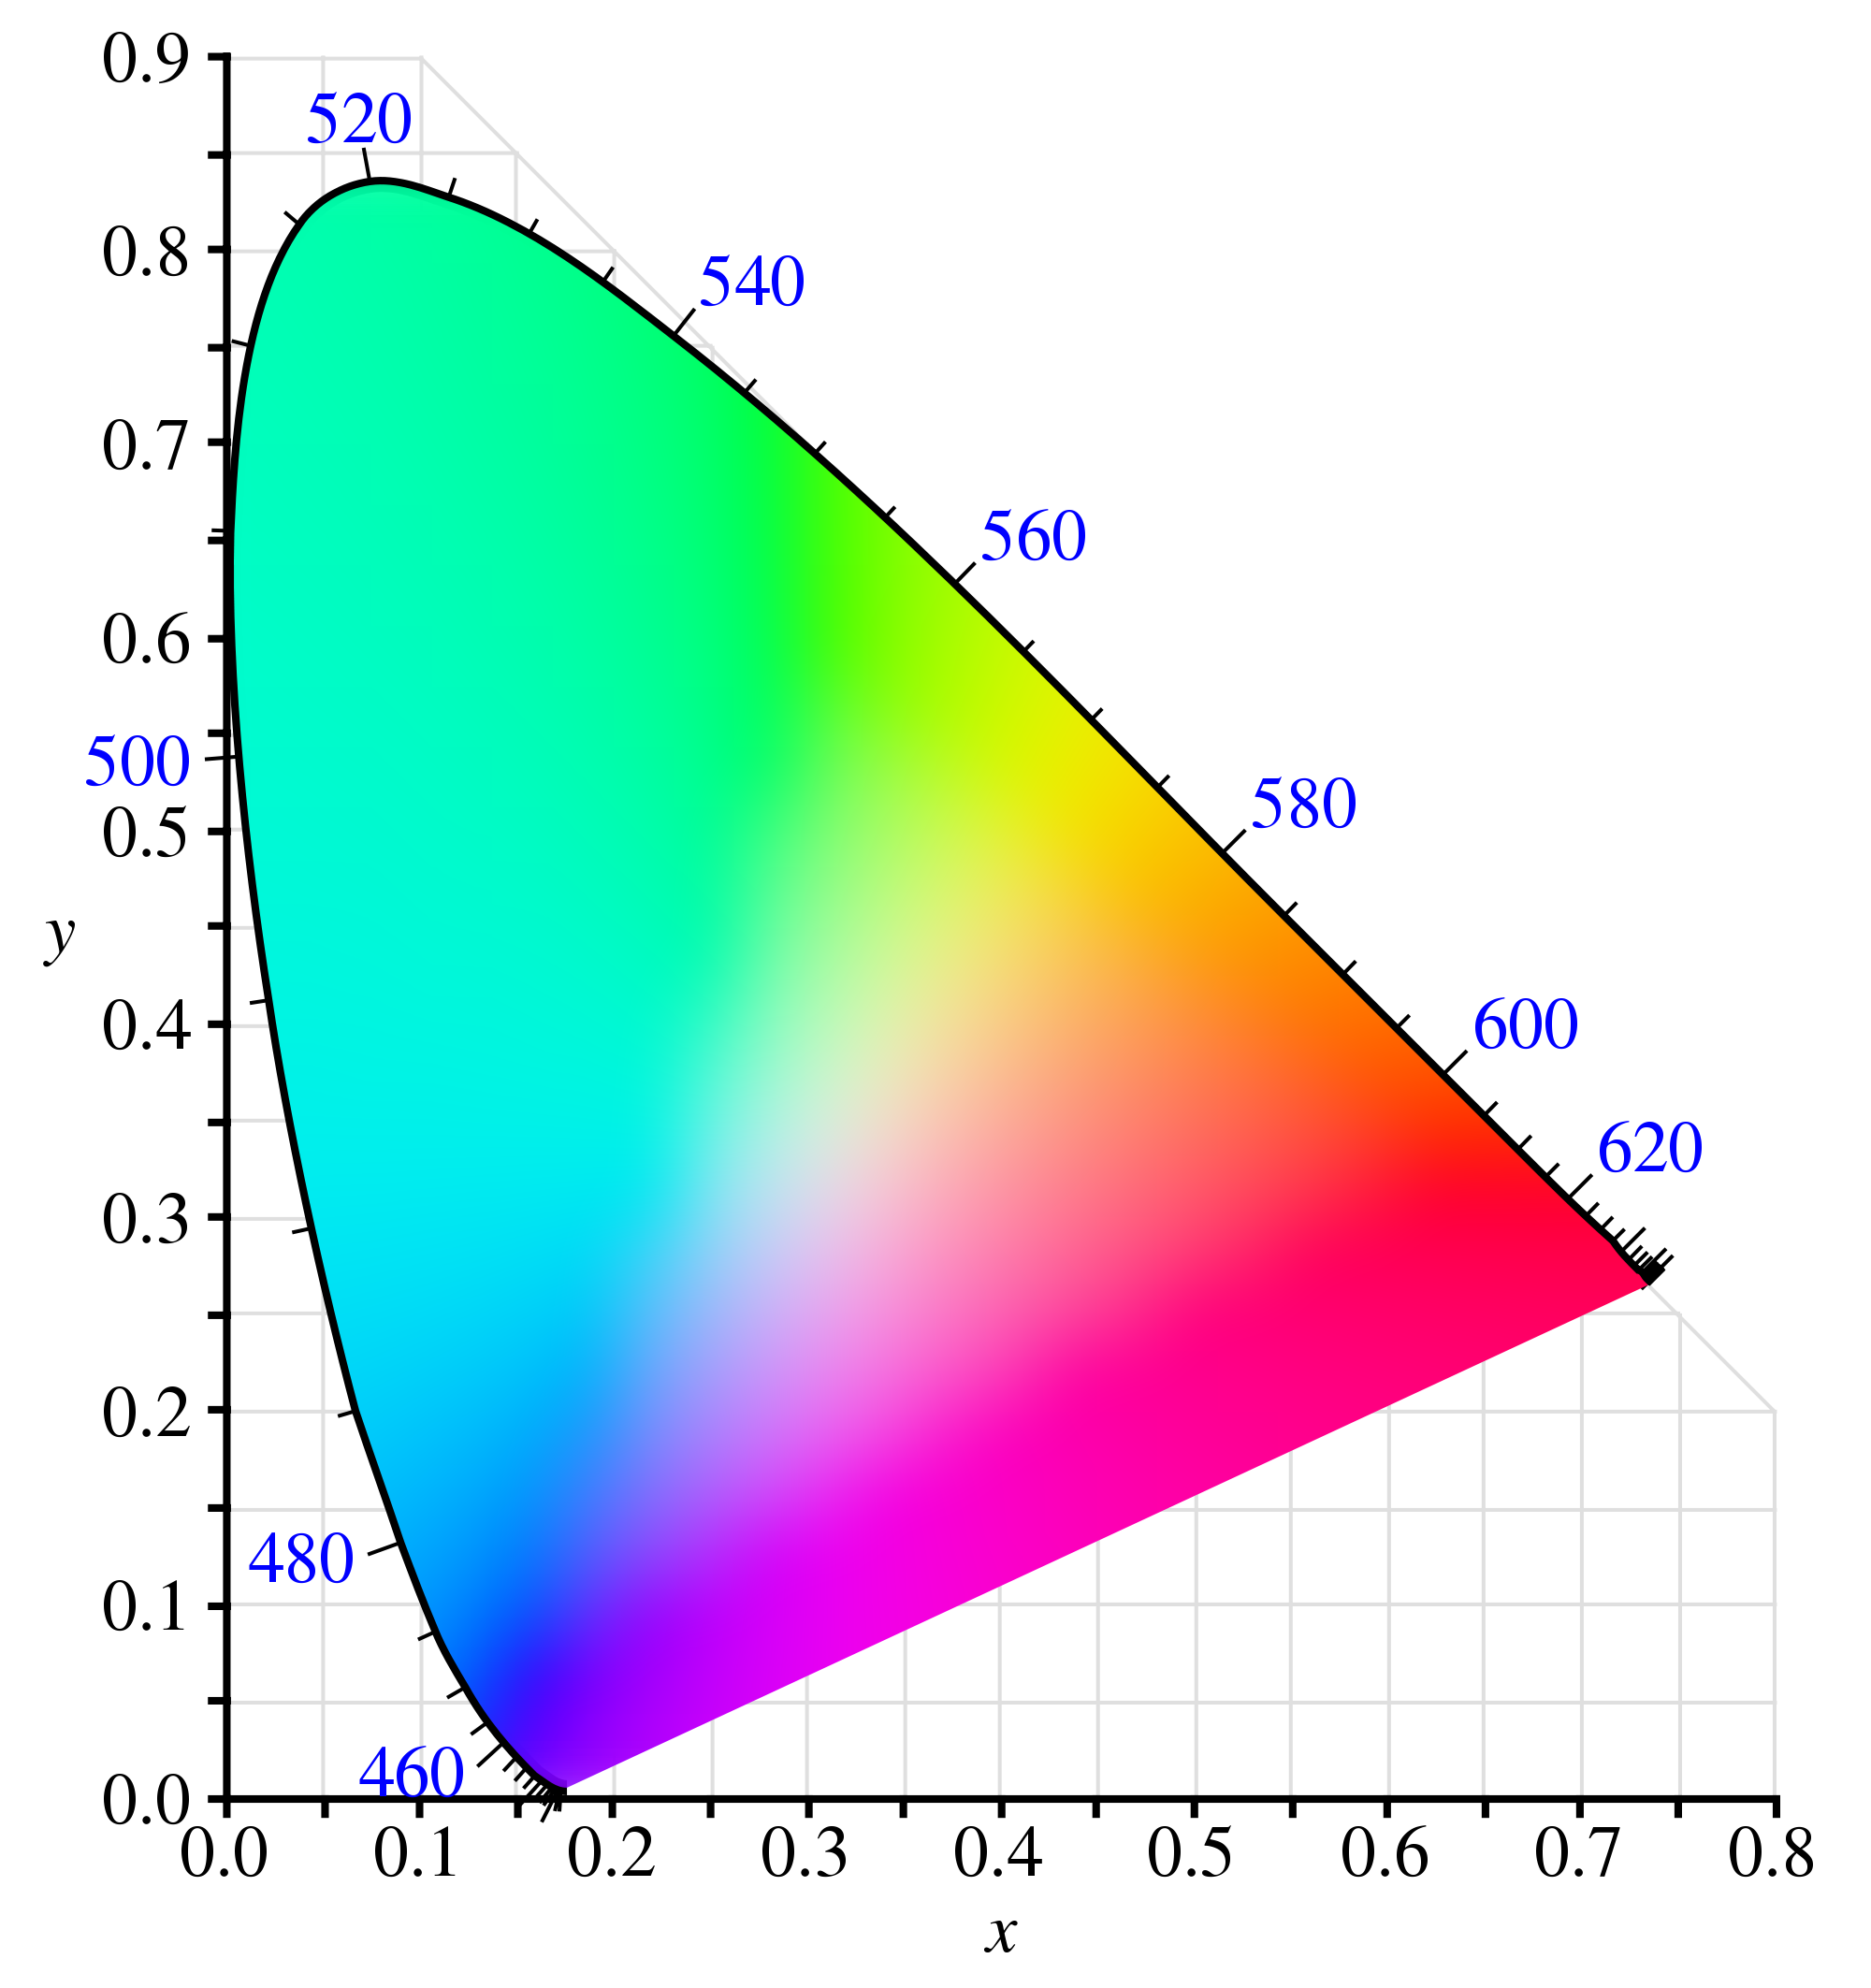
\includegraphics[width =\textwidth]{figure/CIE1931_color_space.png}
% Image from BenRG (https://commons.wikimedia.org/wiki/File:CIE1931xy\_blank.svg), ``CIE1931xy blank", marked as public domain, more details on Wikimedia Commons.
\end{minipage}\hfill
\begin{minipage}{.55\textwidth}
\captionof{figure}{The CIE 1931 colour space chromaticity diagram. The CIE 1931 colour spaces defined the colour space based on physiologically perceived colours in human colour vision. The outer boundary of the curve marks the colour spectrum, with wavelengths in nm. Note that the distance between successive markings on this boundary is not constant, indicating that the perceptual distance between colours does not match the physical distance in wavelength. More broadly, there is much less area devoted to red, orange, yellow, and violet compared to blue and green; as a result, a rainbow colour scheme with equal spacing by wavelength would perceptually over-emphasize the tails of the range of values represented by the scheme.\label{fig:perceptual-colourspace}\vspace{3mm}}
\end{minipage}


While colour is an extremely useful aesthetic for the majority of the population, between 4 and 8 percent of males (and a much smaller proportion of females) have some sort of colour perception deficiency (`colourblindness')~\citep{wakitaSmartColorDisambiguationFramework2005} which reduces the space of distinguishable colours. Colourblindness is common enough that it is reasonable to expect that any given chart used in a presentation or publication will be read by someone who is colour deficient. The use of dual encoding allows colourblind individuals to more readily read graphics which utilize colour, and as hue and lightness can be varied separately, it is possible to use dual-encoding without adding another aesthetic. If accessibility is the goal,
default colors used in ggplot2~\citep{ggplot2} should be avoided, as the saturation is held constant in this color scheme and only the hue of the colors is varied. A perceptually more successful approach to color manipulation can be found in the R package colorspace~\citep{zeileis}. This package is also based on the HCL (Hue, Chroma, Luminance) space of colors, but makes use of both luminance and hue when setting up color schemes and allows an assessment of colors on these three dimensions.
 There are several pre-existing colour schemes which may be more discriminable to colour deficient individuals, such as those provided in \citet{dichromatpackage} or \citet{colorbrewer}. Similarly, when color accessibility of a plot is a primary consideration the use of the default grey background in ggplot2 and other plotting systems should be replaced with white to maximize the contrast between background and plotted features. The default grey background for plots, which by now has become ggplot2's signature look, dates back to a recommendation in \citet{dancarr.grey} to make gridlines in plots readable without dominating the data. Obviously, light grey gridlines on a white background serve the same purpose.

%Where there are no pre-existing associations between variable and colour choice, and colour deficiency is not a concern, evidence \todo{how to cite?} suggests that different categorical colour schemes do not produce significant changes in the perception of the same plot.DHC: I don't think that this is true, might be better to avoid saying, in light of the do no harm principle


\section{OPEN QUESTIONS AND FUTURE RESEARCH} % 3 pages
% We will conclude by identifying promising areas of active research. We will also briefly discuss the use and testing of interactive graphics.

One of the areas in graphics showing the most recent growth and creating the most excitement in the community are interactive graphics.
There are a huge abundance of applications and graphics claiming to be \textit {interactive} - yet then~\citep{debby.interactive} and now there is not much agreement over what `interactive graphics' actually means. While any communication between user and device can be considered an interaction, interactive graphics should be defined as a user-driven direct manipulation of plots and plotting elements with an immediate reaction~\citep{unwin.interactive, becker1987, eick:1995}.
One of the foundations of implementing interactive graphics is the formalization of the data pipeline necessary to support user interactions with the plot~\citep{buja:1988, plumbing, pipeline, cranvas}. The R package \texttt{shiny}~\citep{shiny} is built on this idea; thousands of interactive dashboards and web-applications have been created using that platform.

Formal testing for interactive graphics is difficult without an established and generally accepted grammar of interactive graphics. However, there are several promising approaches into this direction, such as the Python framework vega-lite~\citep{Satyanarayan:cb}, and R packages, e.g.\ \texttt{ggvis}~\citep{ggvis} and \texttt{plotly}~~\citep{plotly}, and most recently \texttt{ggvega}~\citep{ggvega}.
Least well defined in these grammars is usually the aspect of linked brushing and highlighting in plots~\citep{Becker:1987dh}, a technique crucial to interactive graphics for defining and exploring subsets of the data.
An additional problem for interactive graphics is reproducibility of a user's work. By definition, interactive graphics enable a flow, rather than a single static result.
Very recent advances such as trackr~\citep{Becker:2019hp} not only record the user's interactions with the data, but also try to infer the user's intent by collecting metadata and automatically analysing the structure of the data and the code.
This approach might be used in testing, both to evaluate different user's approaches as well as the tools used.

Another open question is the acceptance of results -- a lot of historical research on best practices exists, but how much of it is being put into practice? One does not have to look far to find astonishingly bad graphics in astonishingly good outlets. We are not going to point fingers, here, but will defer to online communities such as \url{https://www.reddit.com/r/dataisugly/} that have passionate discussions on the worst mis-uses of graphics.
%Overall, there are still very large holes in the graphical testing literature, in part because our brains are so complex that it's extremely hard to control for everything but the one effect a single experiment is examining.
What can we do about this? It is up to statisticians to teach more graphics and better graphics in the classroom in the hope to slowly change the climate.
One incentive in the adoption of best practices might be where there is a cost benefit, such as when assessing business performance, or a marketing campaign, there is scope for providing a measure on which to gauge effective visual communication. There is also significant room to improve plots in academic publications in order to better communicate research results~\citep{antony-inpress}.

In the 100 years of empirical evaluation of the perception and utility of statistical graphics, we have assembled a working knowledge of how to best create graphs which are easily read and understood. Once rare, charts are now everywhere we look - on the news, in papers and magazines, and online in interactive form. Going forward, we must do a better job of translating the academic research into practice, making it easier for academics and non-academics alike to create useful, well-designed graphics.

% \section{ACCEPTANCE OF RESULTS} % 3.5 pages
% % There is often a considerable distance between best practice and common practice: researchers have been complaining about pie charts for more than 100 years. We will discuss the acceptance of the results summarized in the previous section, including an examination of persistent offenders, such as pie and candlestick charts, dual axes, dynamite plots.
%
% Tons of historical research, but how much of it has been put into practice? Overall, there are still very large holes in the graphical testing literature, in part because our brains are so complex that it's extremely hard to control for everything but the one effect a single experiment is examining.
%
% % Not sure adding something liek this is useful: That said, there is room for improvement on adoption of best practices. Where there is a cost benefit, such as assessing business performance, or a marketing campaign, there is scope for providing a measure on which to gauge effective visual communication. There is scope in academic publications to to improve plots in published articles.
%
% \section{INTERACTIVE GRAPHICS}
%
% There is huge abundance of applications and graphics calling itself \textit {interactive} - yet then~\citep{debby.interactive} and now there is not much agreement over what `interactive graphics' actually means. While any communication between user and device can be considered an interaction, interactive graphics should be defined as a user-driven direct manipulation of plots and plotting elements with an immediate reaction~\citep{unwin.interactive, becker1987, eick:1995}.
% One of the foundations of implementing interactive graphics is the formalization of the data pipeline necessary to support user interactions with the plot~\citep{buja:1988, plumbing, pipeline, cranvas}. On this basis, the R package shiny~\citep{shiny} is built, which all by itself triggered the creation of thousands of interactive dashboards and web-applications.
%
% Formal testing for interactive graphics is difficult without an established and generally accepted grammar of interactive graphics. However, there are several promising approaches into this direction, such as the Python framework vega-lite~\citep{Satyanarayan:cb}, and R packages, e.g.\ ggvis~\citep{ggvis} and plotly~\citep{plotly}, and most recently ggvega~\citep{ggvega}.
%
% Least well defined in these grammars is usually the aspect of linked brushing and highlighting in plots~\citep{Becker:1987dh}, a technique crucial to interactive graphics for defining and exploring subsets of the data.
%
% An additional problem for interactive graphics is reproducibility of a user's work. By definition, interactive graphics enable a flow, rather than a single static result.
% Very recent advances such as trackr~\citep{Becker:2019hp} not only script the user's interactions with the data, but also try to infer the user's intent by collecting metadata and automatically analysing the structure of the data and the code.
% This approach might be used in testing, both to evaluate different user's approaches as well as the tools used.
%
%
% \section{OPEN QUESTIONS AND FUTURE RESEARCH} % 3 pages
% % We will conclude by identifying promising areas of active research. We will also briefly discuss the use and testing of interactive graphics.
%
% As cognitive perception research has advanced so dramatically, transitioning what has been learned into improving data plotting practices would be a fruitful direction.
%
% A data plot is not designed to compete with numerical statistics. If accuracy is what is of interest, showing the data as a table is clearly preferable. Techniques to be able to quantify effectiveness of plots in ways other than accuracy and speed are needed.

%Disclosure
\section*{DISCLOSURE STATEMENT}
% If the authors have noting to disclose, the following statement will be used:
The authors are not aware of any affiliations, memberships, funding, or financial holdings that
might be perceived as affecting the objectivity of this review.

% Acknowledgements
\section*{ACKNOWLEDGMENTS}
% Acknowledgements, general annotations, funding.
Heike Hofmann and Susan Vanderplas are partially supported by the Center for Statistics and Applications in Forensic Evidence (CSAFE) through Cooperative Agreement \#70NANB15H176 between NIST and Iowa State University, which includes activities carried out at Carnegie Mellon University, University of California Irvine, and University of Virginia.
\clearpage
% \section*{REFERENCES}
\bibliography{references}

\end{document}
% %Example of a Figure
% \section{ELEMENTS\ OF\ THE\ MANUSCRIPT}
% \subsection{Figures}Figures should be cited in the main text in chronological order. This is dummy text with a citation to the first figure (\textbf{Figure \ref{fig1}}). Citations to \textbf{Figure \ref{fig1}} (and other figures) will be bold.
%
% \begin{figure}[h]
% 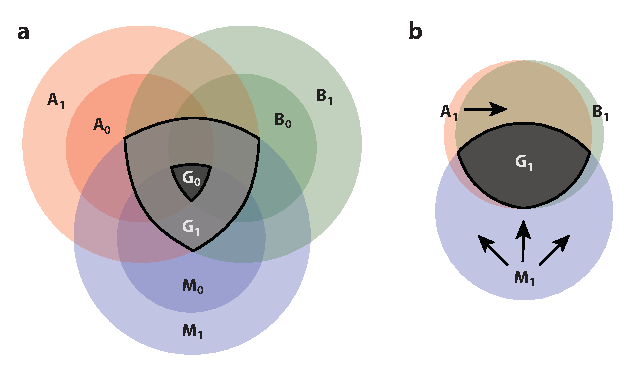
\includegraphics[width=3in]{SampleFigure}
% \caption{Figure caption with descriptions of parts a and b}
% \label{fig1}
% \end{figure}
%
% % Example of a Table
% \subsection{Tables} Tables should also be cited in the main text in chronological order (\textbf {Table \ref{tab1}}).
%
% \begin{table}[h]
% \tabcolsep7.5pt
% \caption{Table caption}
% \label{tab1}
% \begin{center}
% \begin{tabular}{@{}l|c|c|c|c@{}}
% \hline
% Head 1 &&&&Head 5\\
% {(}units)$^{\rm a}$ &Head 2 &Head 3 &Head 4 &{(}units)\\
% \hline
% Column 1 &Column 2 &Column3$^{\rm b}$ &Column4 &Column\\
% Column 1 &Column 2 &Column3 &Column4 &Column\\
% Column 1 &Column 2 &Column3 &Column4 &Column\\
% Column 1 &Column 2 &Column3 &Column4 &Column\\
% \hline
% \end{tabular}
% \end{center}
% \begin{tabnote}
% $^{\rm a}$Table footnote; $^{\rm b}$second table footnote.
% \end{tabnote}
% \end{table}
%
% % Example of lists
% \subsection{Lists and Extracts} Here is an example of a numbered list:
% \begin{enumerate}
% \item List entry number 1,
% \item List entry number 2,
% \item List entry number 3,\item List entry number 4, and
% \item List entry number 5.
% \end{enumerate}
%
% Here is an example of a extract.
% \begin{extract}
% This is an example text of quote or extract.
% This is an example text of quote or extract.
% \end{extract}
%
% \subsection{Sidebars and Margin Notes}
% % Margin Note
% \begin{marginnote}[]
% \entry{Term A}{definition}
% \entry{Term B}{definition}
% \entry{Term C}{defintion}
% \end{marginnote}
%
% \begin{textbox}[h]\section{SIDEBARS}
% Sidebar text goes here.
% \subsection{Sidebar Second-Level Heading}
% More text goes here.\subsubsection{Sidebar third-level heading}
% Text goes here.\end{textbox}
%
%
%
% \subsection{Equations}
% % Example of a single-line equation
% \begin{equation}
% a = b \ {\rm ((Single\ Equation\ Numbered))}
% \end{equation}
% %Example of multiple-line equation
% Equations can also be multiple lines as shown in Equations 2 and 3.
% \begin{eqnarray}
% c = 0 \ {\rm ((Multiple\  Lines, \ Numbered))}\\
% ac = 0 \ {\rm ((Multiple \ Lines, \ Numbered))}
% \end{eqnarray}
%
% % Summary Points
% \begin{summary}[SUMMARY POINTS]
% \begin{enumerate}
% \item Summary point 1. These should be full sentences.
% \item Summary point 2. These should be full sentences.
% \item Summary point 3. These should be full sentences.
% \item Summary point 4. These should be full sentences.
% \end{enumerate}
% \end{summary}
%
% % Future Issues
% \begin{issues}[FUTURE ISSUES]
% \begin{enumerate}
% \item Future issue 1. These should be full sentences.
% \item Future issue 2. These should be full sentences.
% \item Future issue 3. These should be full sentences.
% \item Future issue 4. These should be full sentences.
% \end{enumerate}
% \end{issues}


% % References
% %
% % Margin notes within bibliography
% \section*{LITERATURE\ CITED}
%
% To download the appropriate bibliography style file, please see \url{http://www.annualreviews.org/page/authors/author-instructions/preparing/latex}. \\
%
% \noindent
% Please see the Style Guide document for instructions on preparing your Literature Cited.
%
% The citations should be listed in alphabetical order, with titles. For example:
%
%
%
%
%
%
% \begin{verbatim}
% \begin{thebibliography}{00}
% \bibitem[Acevedo \& Fitzjarrald(2001)]{Acevedo:01}
% Acevedo O, Fitzjarrald D. 2001.
% The early evening surface-layer transition: temporal and spatial variability.
% \textit{J. Atmos. Sci.} 58:2650--67
%
% \bibitem[Acevedo et~al.(2009)Acevedo, Moraes, Degrazia, Fitzjarrald, Manzi \&
%   Campos]{Acevedo:09}
% Acevedo O, Moraes O, Degrazia G, Fitzjarrald D, Manzi A, Campos J. 2009.
% Is friction velocity the most appropriate scale for correcting nocturnal carbon
%   dioxide fluxes?
% \textit{Agric. For. Meteorol.} 149:1--10
%
% \bibitem[Baas et~al.(2006)Baas, Steeneveld, {van de Weil} \& Holtslag]{Baas:09}
% Baas P, Steeneveld G, {van de Weil} B, Holtslag A. 2006.
% Exploring self-correlation in the flux-gradient relationships for stably
%   stratified conditions.
% \textit{J. Atmos. Sci.} 63:3045--54
%
% \bibitem[Badran, Thiria \& Crepon(1991)]{Badran:91}
% Badran F, Thiria S, Crepon M. 1991.
% Wind ambiguity removal by the use of neural network techniques.
% \textit{J. Geophys. Res.} 96:20,521--29
%
% \bibitem[Bakas \& Ioannou(2007)]{Bakas:07}
% Bakas NA, Ioannou PJ. 2007.
% Momentum and energy transport by gravity waves in stochastically driven
%   stratified flows. {Part I}: radiation of gravity waves from a shear layer.
% \textit{J. Atmos. Sci.} 64:1509--29
%
% \bibitem[Calanca, Forrer \& Rotach(1998)]{Calanca:98}
% Calanca P, Forrer J, Rotach M. 1998.
% Toward an integral formulation of the turbulent transfer in a stably stratified
%   boundary layer over an ice sheet.
% \textit{Q. J. R. Meteorol. Soc.} 124:1--18
%
% \bibitem[D'Asaro \& Lien(2000)]{DAsaro:00}
% D'Asaro EA, Lien RC. 2000.
% The wave-turbulence transition for stratified flows.
% \textit{J. Phys. Oceanog.} 30:123--45
%
% \bibitem[de~Silva et~al.(1996)de~Silva, Fernando, Eaton \& Hebert]{deSilva:96}
% de~Silva I, Fernando H, Eaton F, Hebert D. 1996.
% Evolution of kelvin-helmholtz billows in nature and laboratory.
% \textit{Earth Planetary Sci. Let.} 143:217--31
%
%
% \end{thebibliography}
% \end{verbatim}
%
%
%
%
% \begin{thebibliography}{00}
%
% \bibitem[Acevedo \& Fitzjarrald(2001)]{Acevedo:01}
% Acevedo O, Fitzjarrald D. 2001.
% The early evening surface-layer transition: temporal and spatial variability.
% \textit{J. Atmos. Sci.} 58:2650--67
%
% \bibitem[Acevedo et~al.(2009)Acevedo, Moraes, Degrazia, Fitzjarrald, Manzi \&
%   Campos]{Acevedo:09}
% Acevedo O, Moraes O, Degrazia G, Fitzjarrald D, Manzi A, Campos J. 2009.
% Is friction velocity the most appropriate scale for correcting nocturnal carbon
%   dioxide fluxes?
% \textit{Agric. For. Meteorol.} 149:1--10
%
% \bibitem[Baas et~al.(2006)Baas, Steeneveld, {van de Weil} \& Holtslag]{Baas:09}
% Baas P, Steeneveld G, {van de Weil} B, Holtslag A. 2006.
% Exploring self-correlation in the flux-gradient relationships for stably
%   stratified conditions.
% \textit{J. Atmos. Sci.} 63:3045--54
%
% \bibitem[Badran, Thiria \& Crepon(1991)]{Badran:91}
% Badran F, Thiria S, Crepon M. 1991.
% Wind ambiguity removal by the use of neural network techniques.
% \textit{J. Geophys. Res.} 96:20,521--29
%
% \bibitem[Bakas \& Ioannou(2007)]{Bakas:07}
% Bakas NA, Ioannou PJ. 2007.
% Momentum and energy transport by gravity waves in stochastically driven
%   stratified flows. {Part I}: radiation of gravity waves from a shear layer.
% \textit{J. Atmos. Sci.} 64:1509--29
%
% \bibitem[Calanca, Forrer \& Rotach(1998)]{Calanca:98}
% Calanca P, Forrer J, Rotach M. 1998.
% Toward an integral formulation of the turbulent transfer in a stably stratified
%   boundary layer over an ice sheet.
% \textit{Q. J. R. Meteorol. Soc.} 124:1--18
%
% \bibitem[D'Asaro \& Lien(2000)]{DAsaro:00}
% D'Asaro EA, Lien RC. 2000.
% The wave-turbulence transition for stratified flows.
% \textit{J. Phys. Oceanog.} 30:123--45
%
% \bibitem[de~Silva et~al.(1996)de~Silva, Fernando, Eaton \& Hebert]{deSilva:96}
% de~Silva I, Fernando H, Eaton F, Hebert D. 1996.
% Evolution of kelvin-helmholtz billows in nature and laboratory.
% \textit{Earth Planetary Sci. Let.} 143:217--31
%
%
%
% \end{thebibliography}
